\chapter{Drone Design and Construction}

\begin{figure}[H]
\begin{subfigure}{0.5\textwidth}
\centering
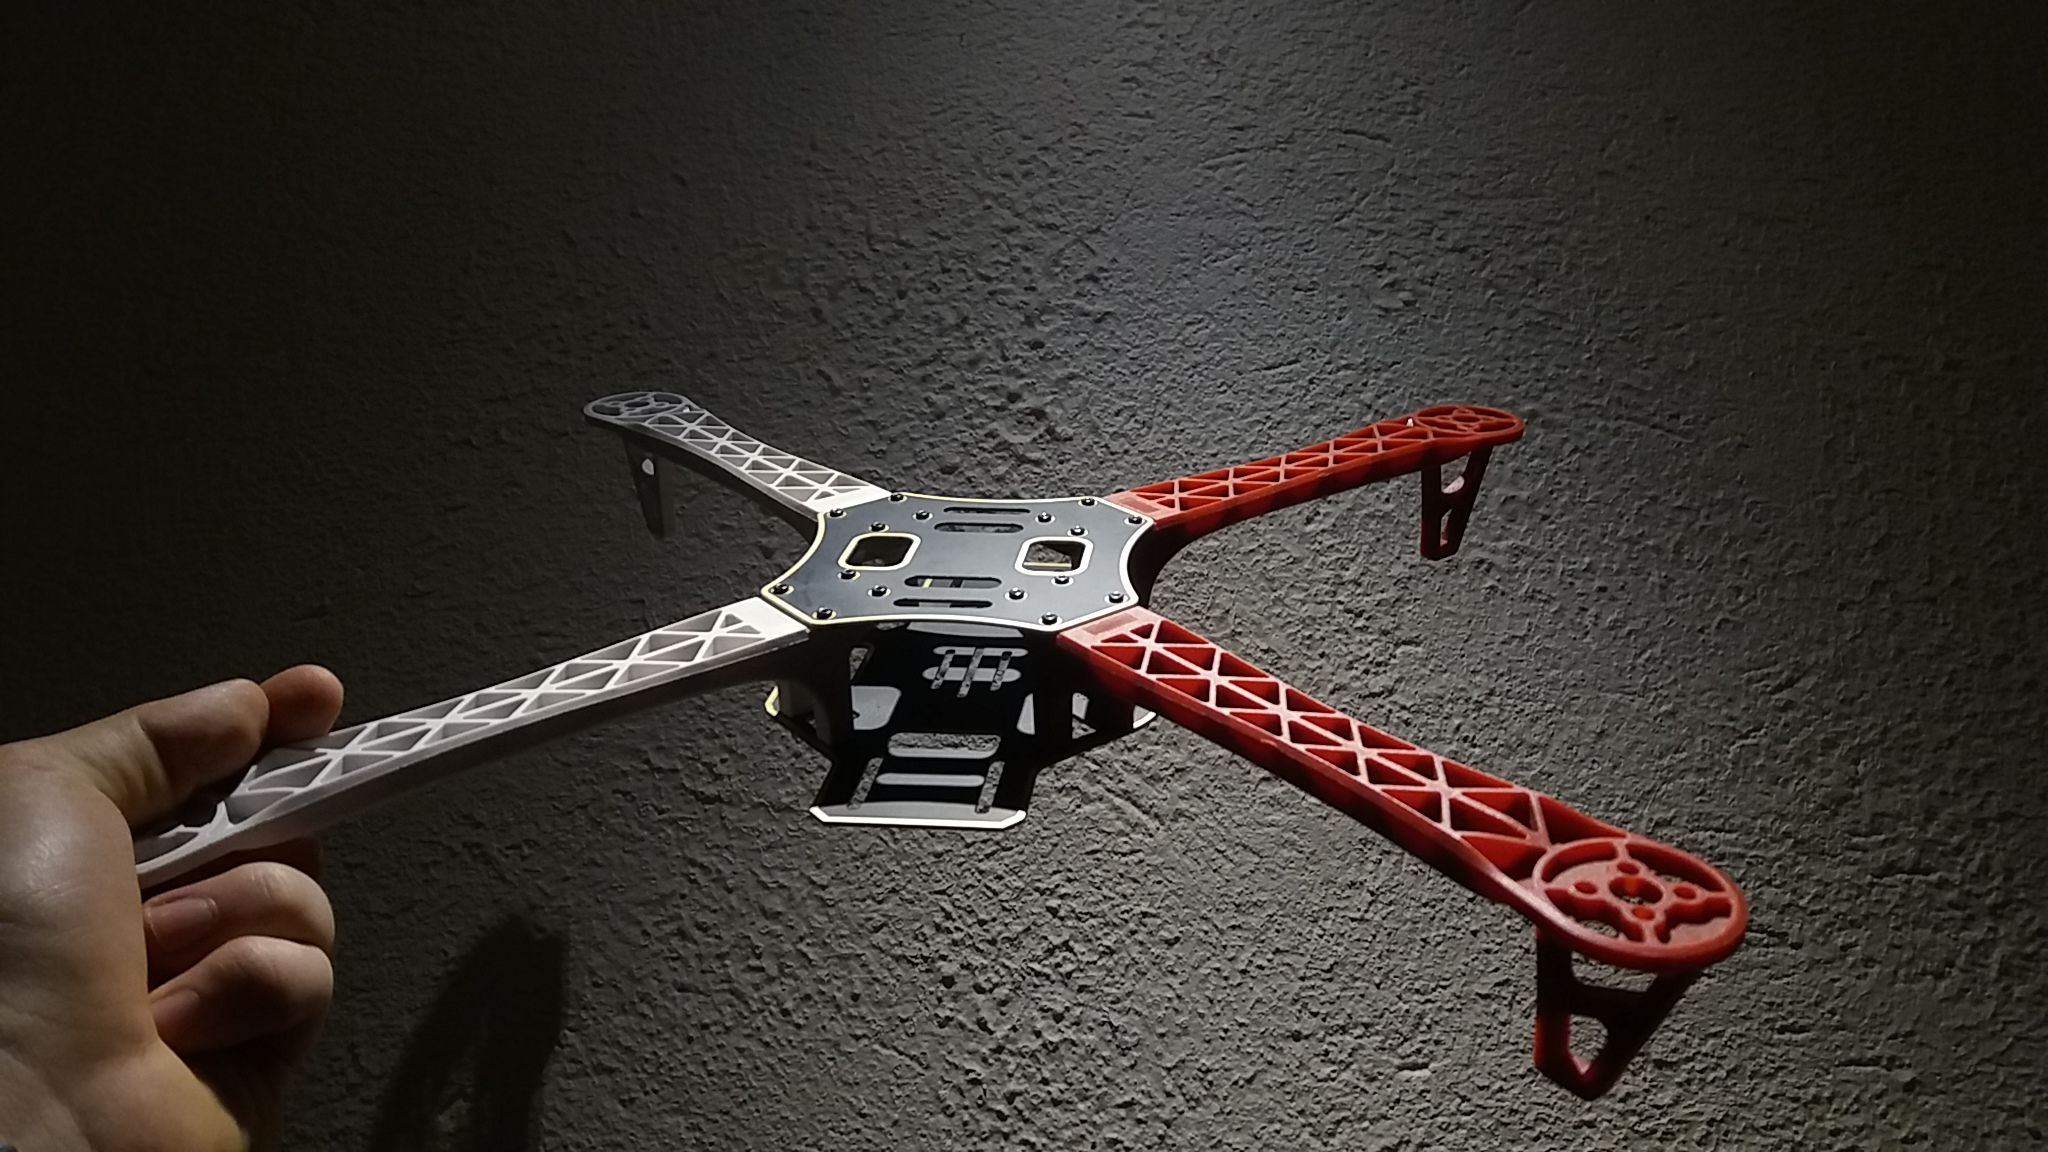
\includegraphics[scale=0.1]{images/drone-build-frame.jpg}
\caption{F450 frame.}
% Reproduced from \cite{gopher}}
\label{fig:frame}
\end{subfigure}
\begin{subfigure}{0.5\textwidth}
\centering
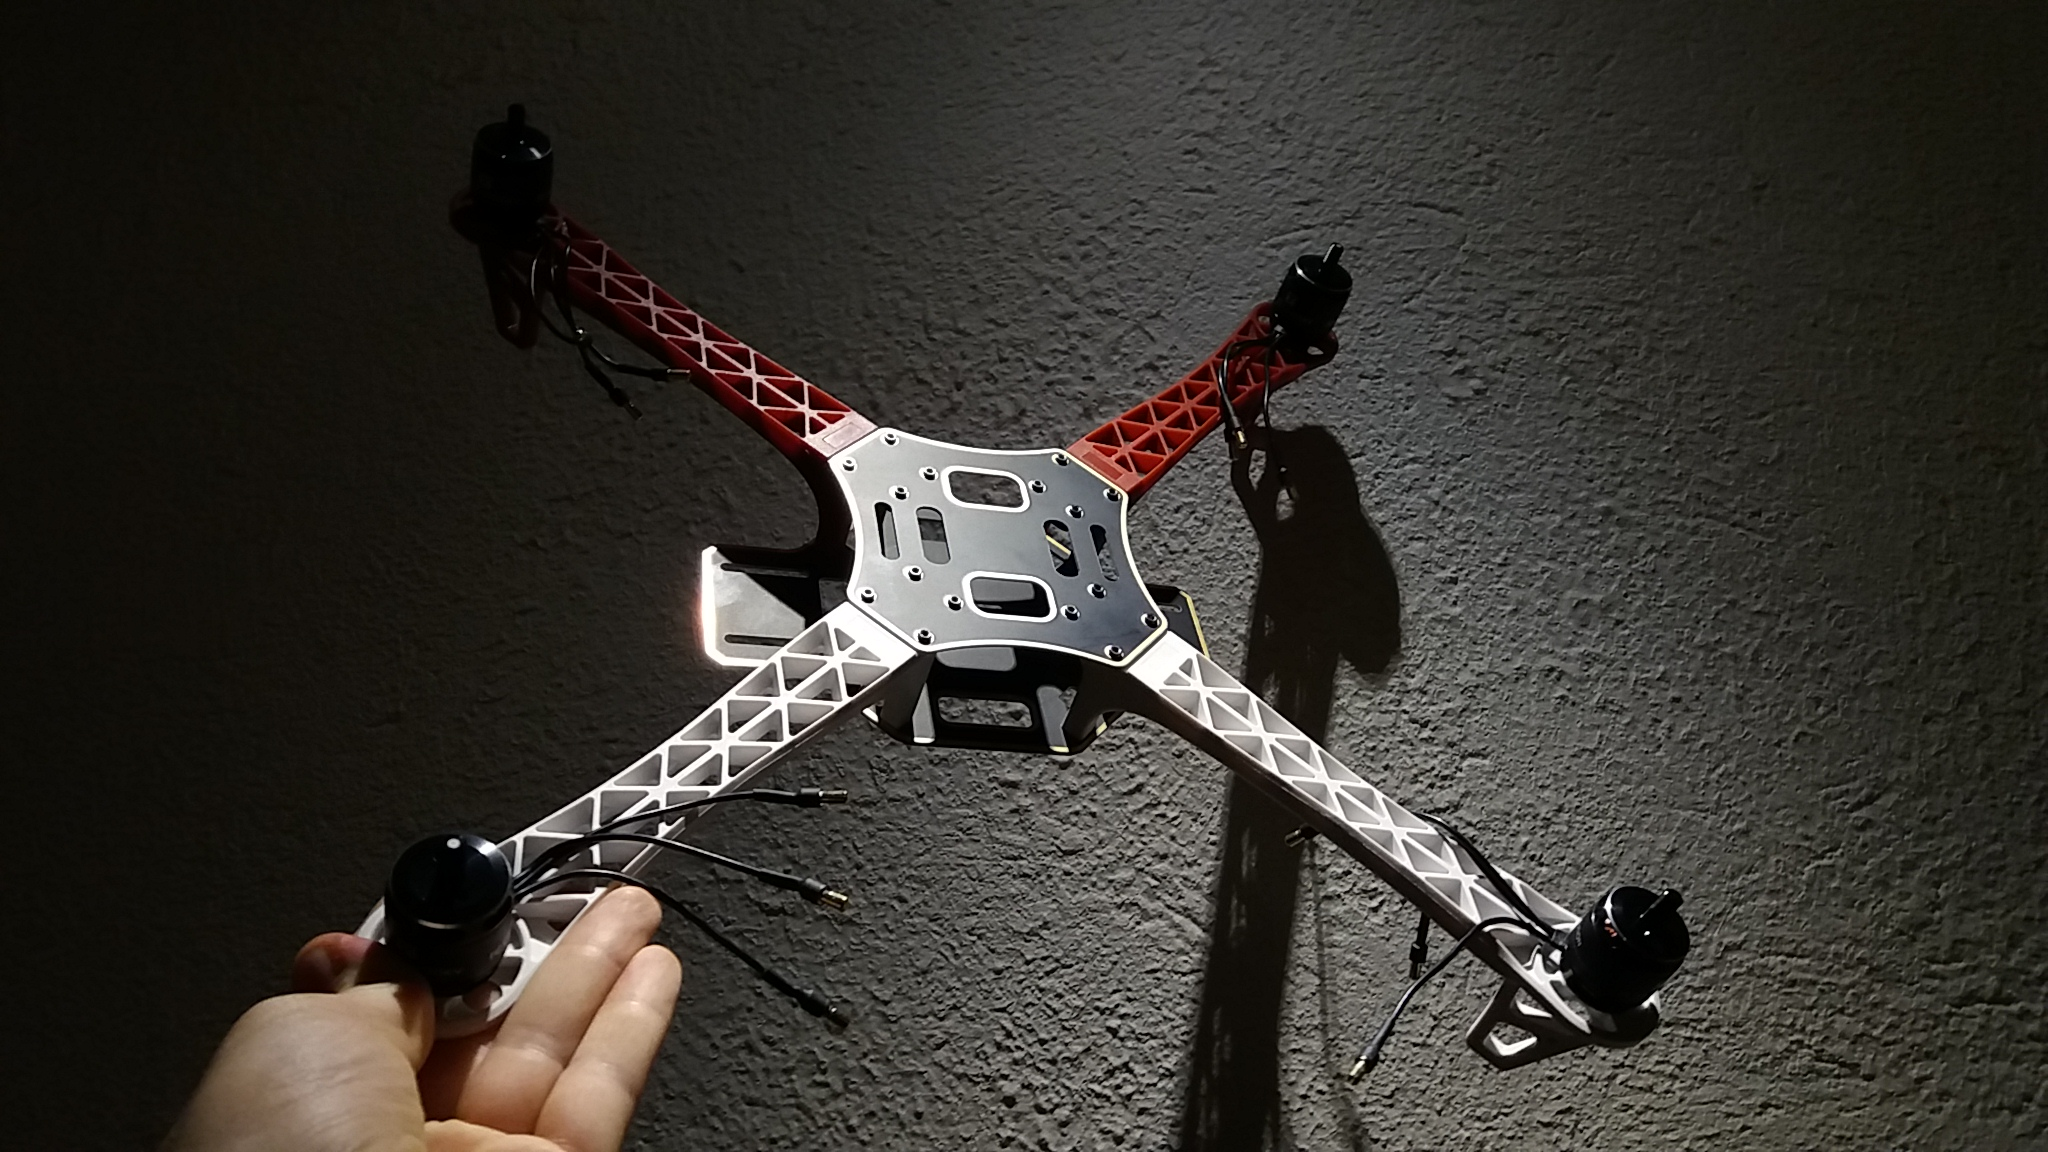
\includegraphics[scale=0.1]{images/drone-build-motors.jpg}
\caption{Adding the 920kv motors.}
\label{fig:motors}
\end{subfigure}
\caption{Frame and motors}
\label{fig:frame_motors}
\end{figure}

\noindent
The frame is made out of a polycarbonate as in Figure \ref{fig:frame}.\\

\begin{figure}[H]
\begin{subfigure}{0.5\textwidth}
\centering
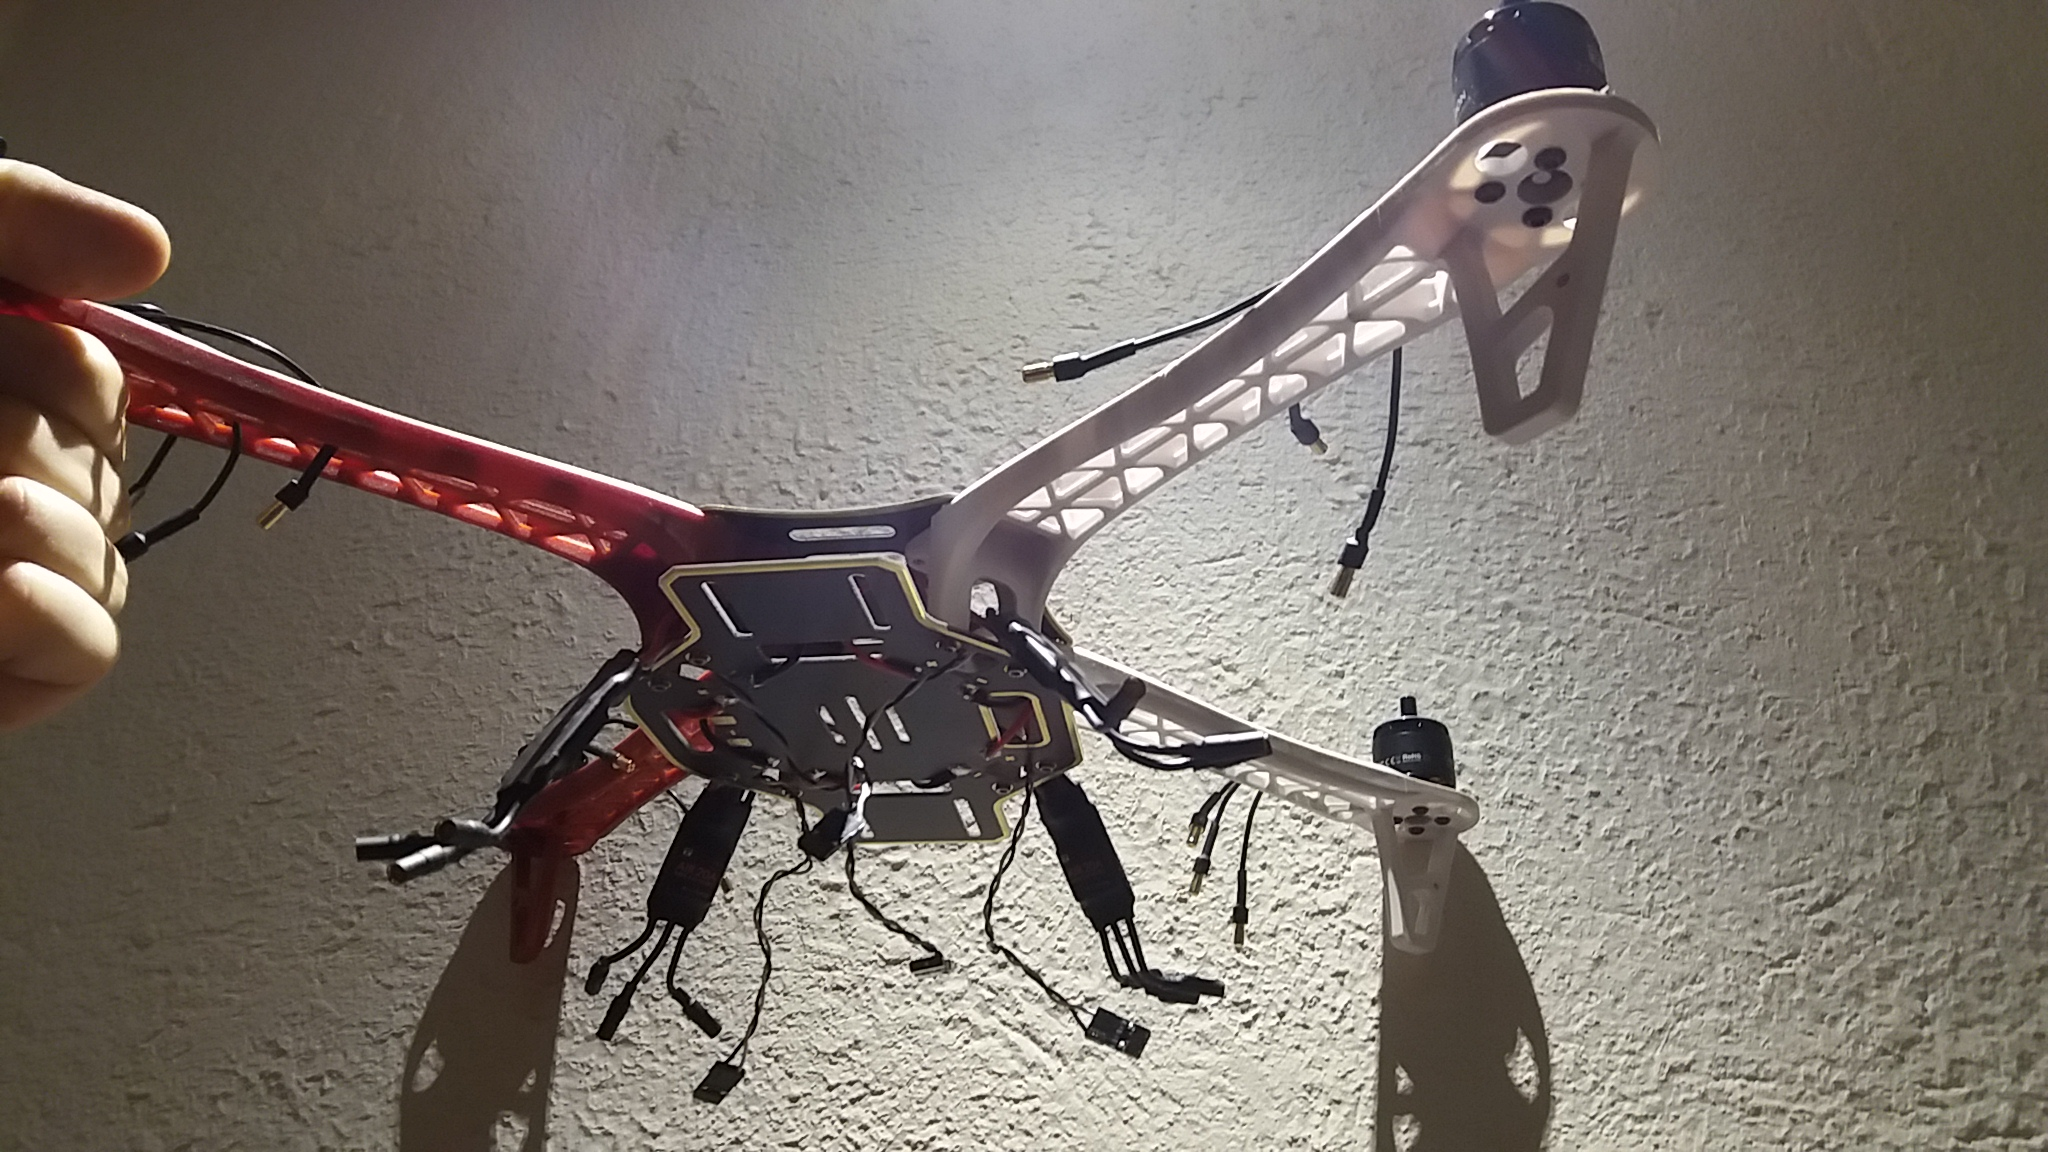
\includegraphics[scale=0.1]{images/drone-build-esc-3phaseunconnected.jpg}
\caption{Adding the ESCs. Motors require 3-phase power}
\label{fig:ESCs_uplugged}
\end{subfigure}
\begin{subfigure}{0.5\textwidth}
\centering
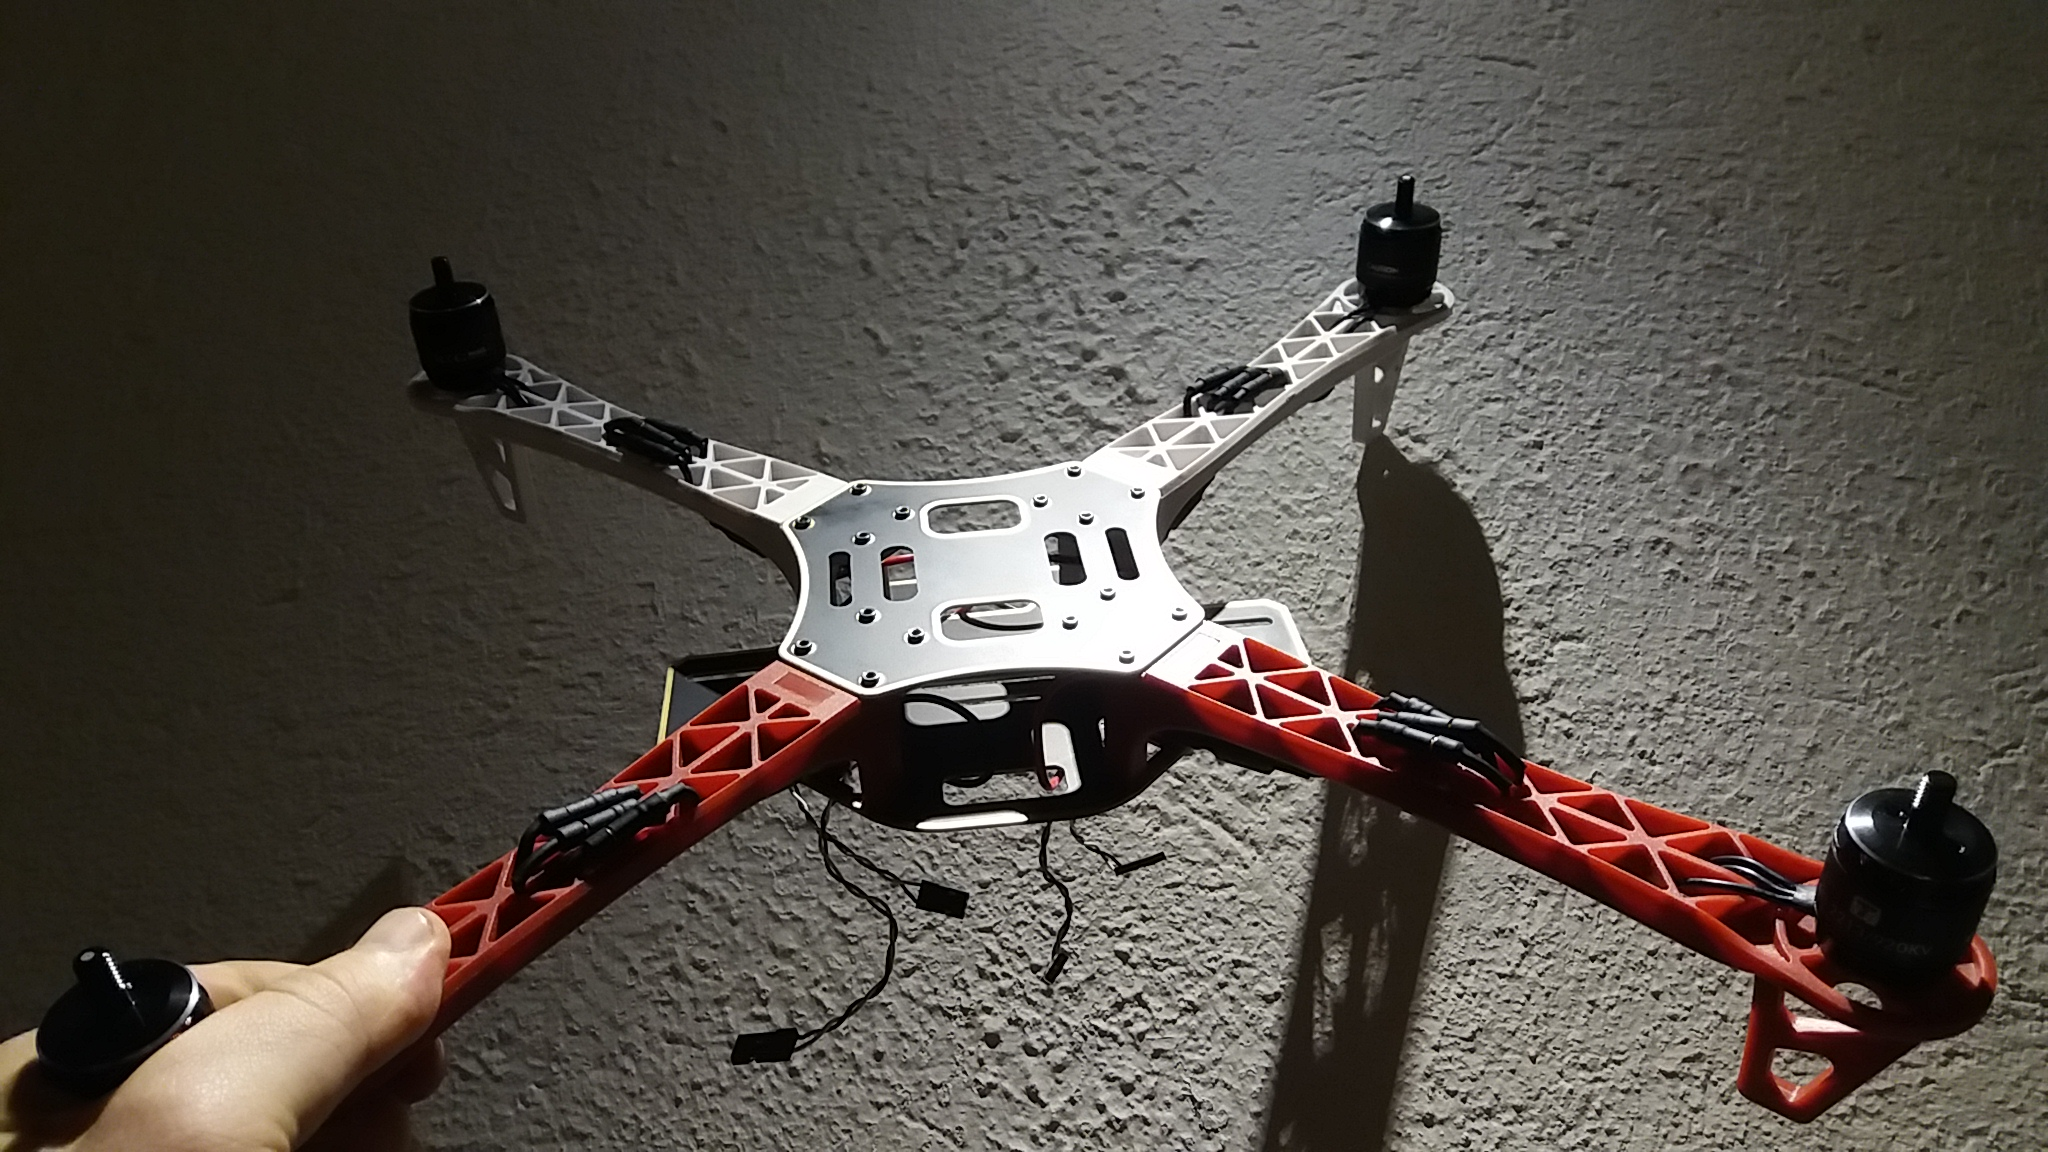
\includegraphics[scale=0.1]{images/drone-build-esc-3phaseconnected.jpg}
\caption{Power leads plugged in and secured}
\label{fig:ESCs_plugged}
\end{subfigure}
\caption{ESCs}
\label{fig:ESC}
\end{figure}

\noindent
The leads are easy to plug/unplug. Any two phase leads can be swapped to change motor direction as in Figure \ref{fig:ESC}.\\

\begin{figure}[H]
\begin{subfigure}{0.5\textwidth}
\centering
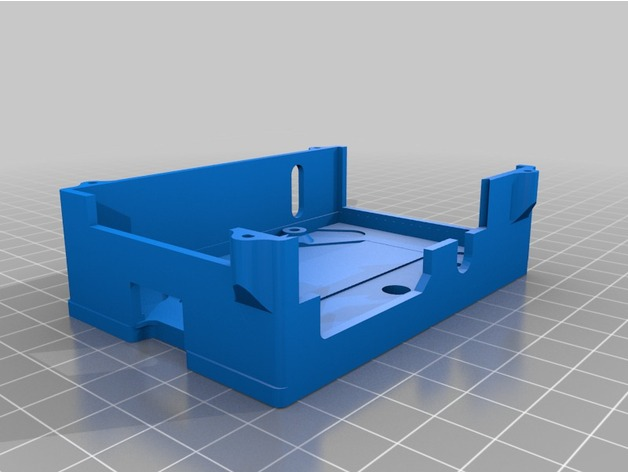
\includegraphics[scale=0.25]{images/drone-build-3d-case-render.jpg}
\caption{Case render}
\label{fig:fcarpc1}
\end{subfigure}
\begin{subfigure}{0.5\textwidth}
\centering
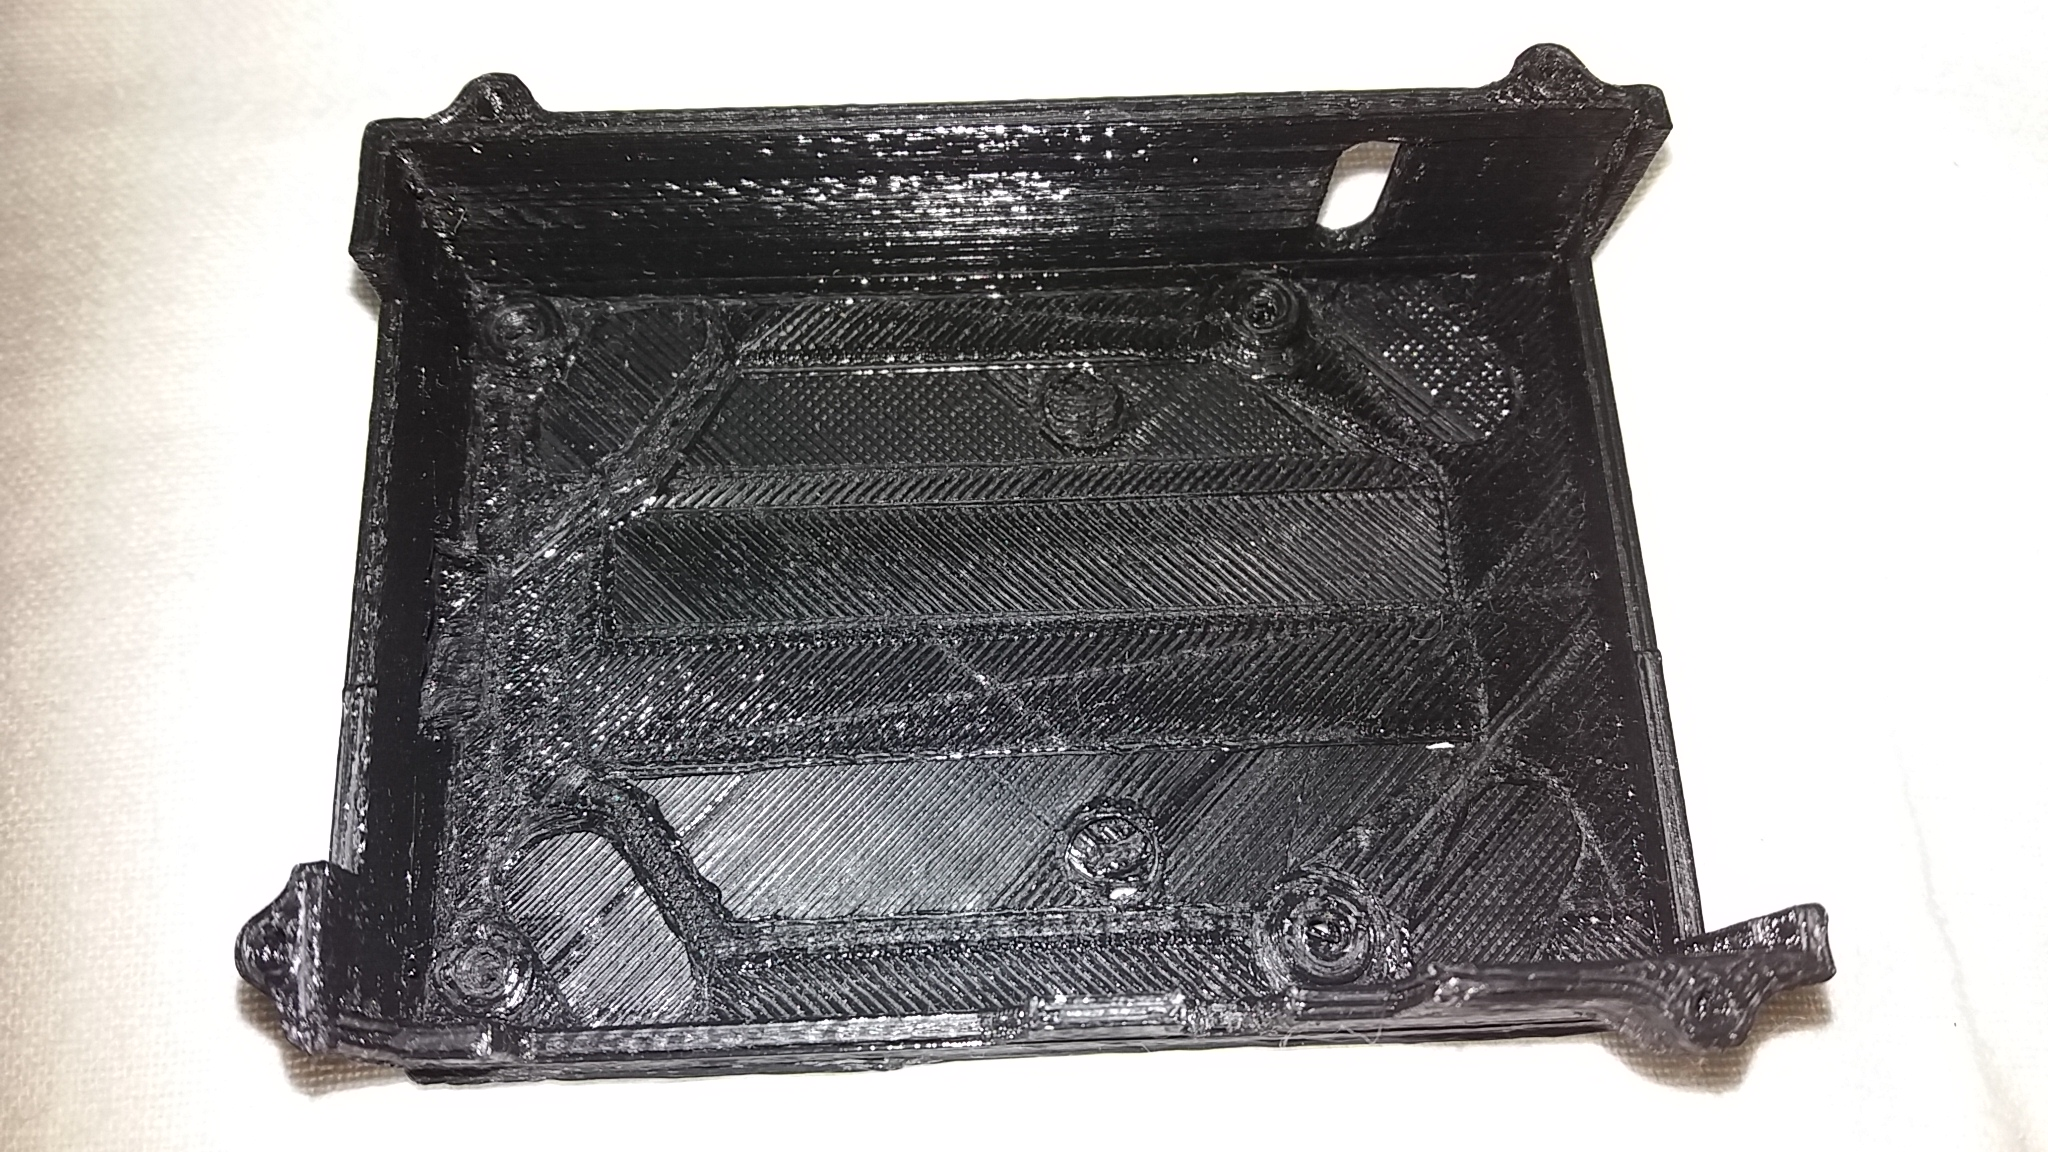
\includegraphics[scale=0.1]{images/drone-build-3dcase.jpg}
\caption{3D printed case for Raspberry Pi and Navio2.}
\label{fcarpc2}
\end{subfigure}
\caption{Flight controller and Raspberry Pi case}
\label{fig:fcarpc}
\end{figure}

\noindent
A housing is needed to protect the exposed electronics from the elements as shown in Figure \ref{fig:fcarpc}. Also, dramatic airflow can affect the barometer readings. Thus, a 3D printed case was made.

\begin{figure}[H]
\begin{subfigure}{0.5\textwidth}
\centering
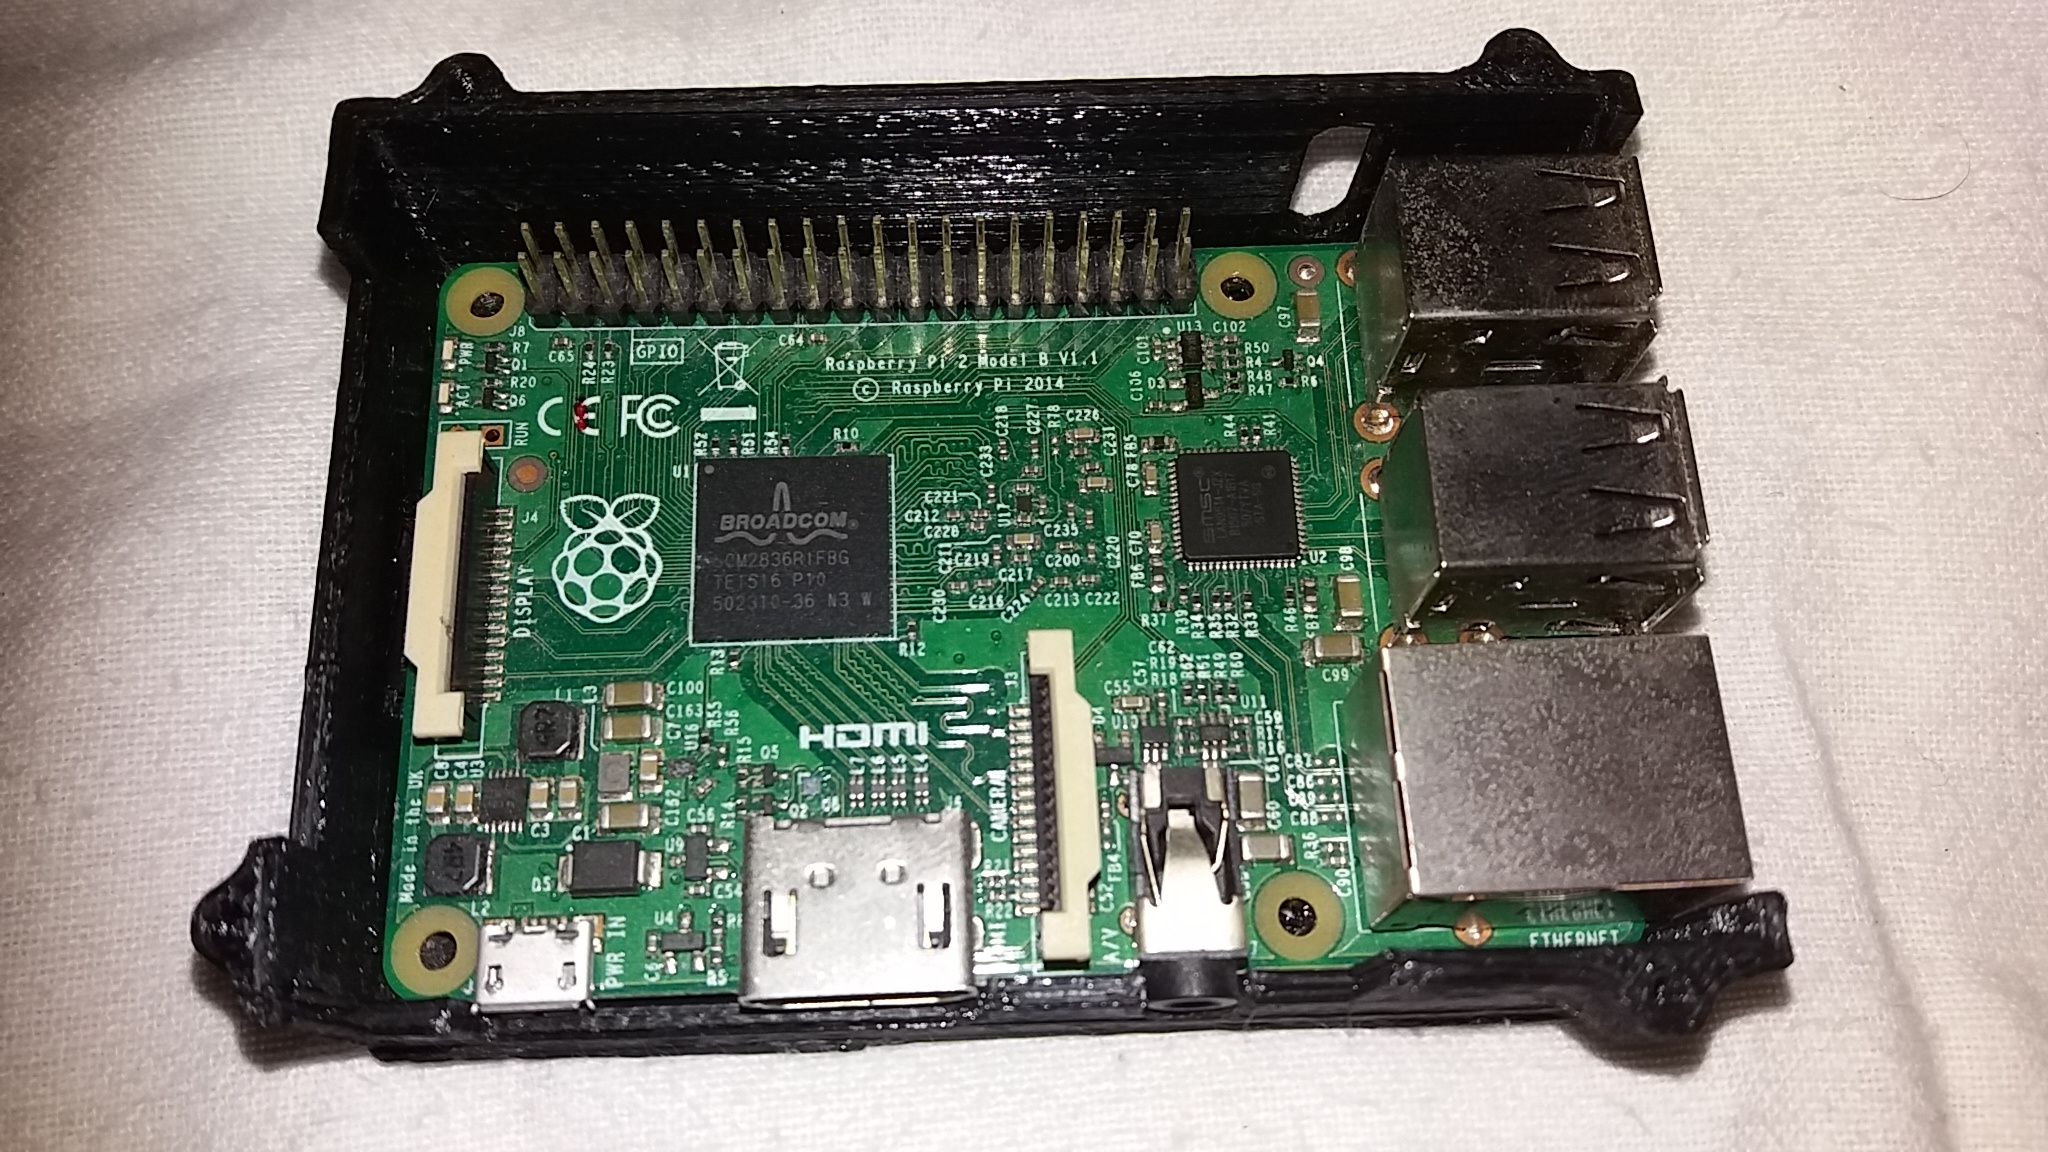
\includegraphics[scale=0.1]{images/drone-build-3dcase-pi.jpg}
\caption{Putting the Pi in the case.}
\label{fig:insertion_pi}
\end{subfigure}
\begin{subfigure}{0.5\textwidth}
\centering
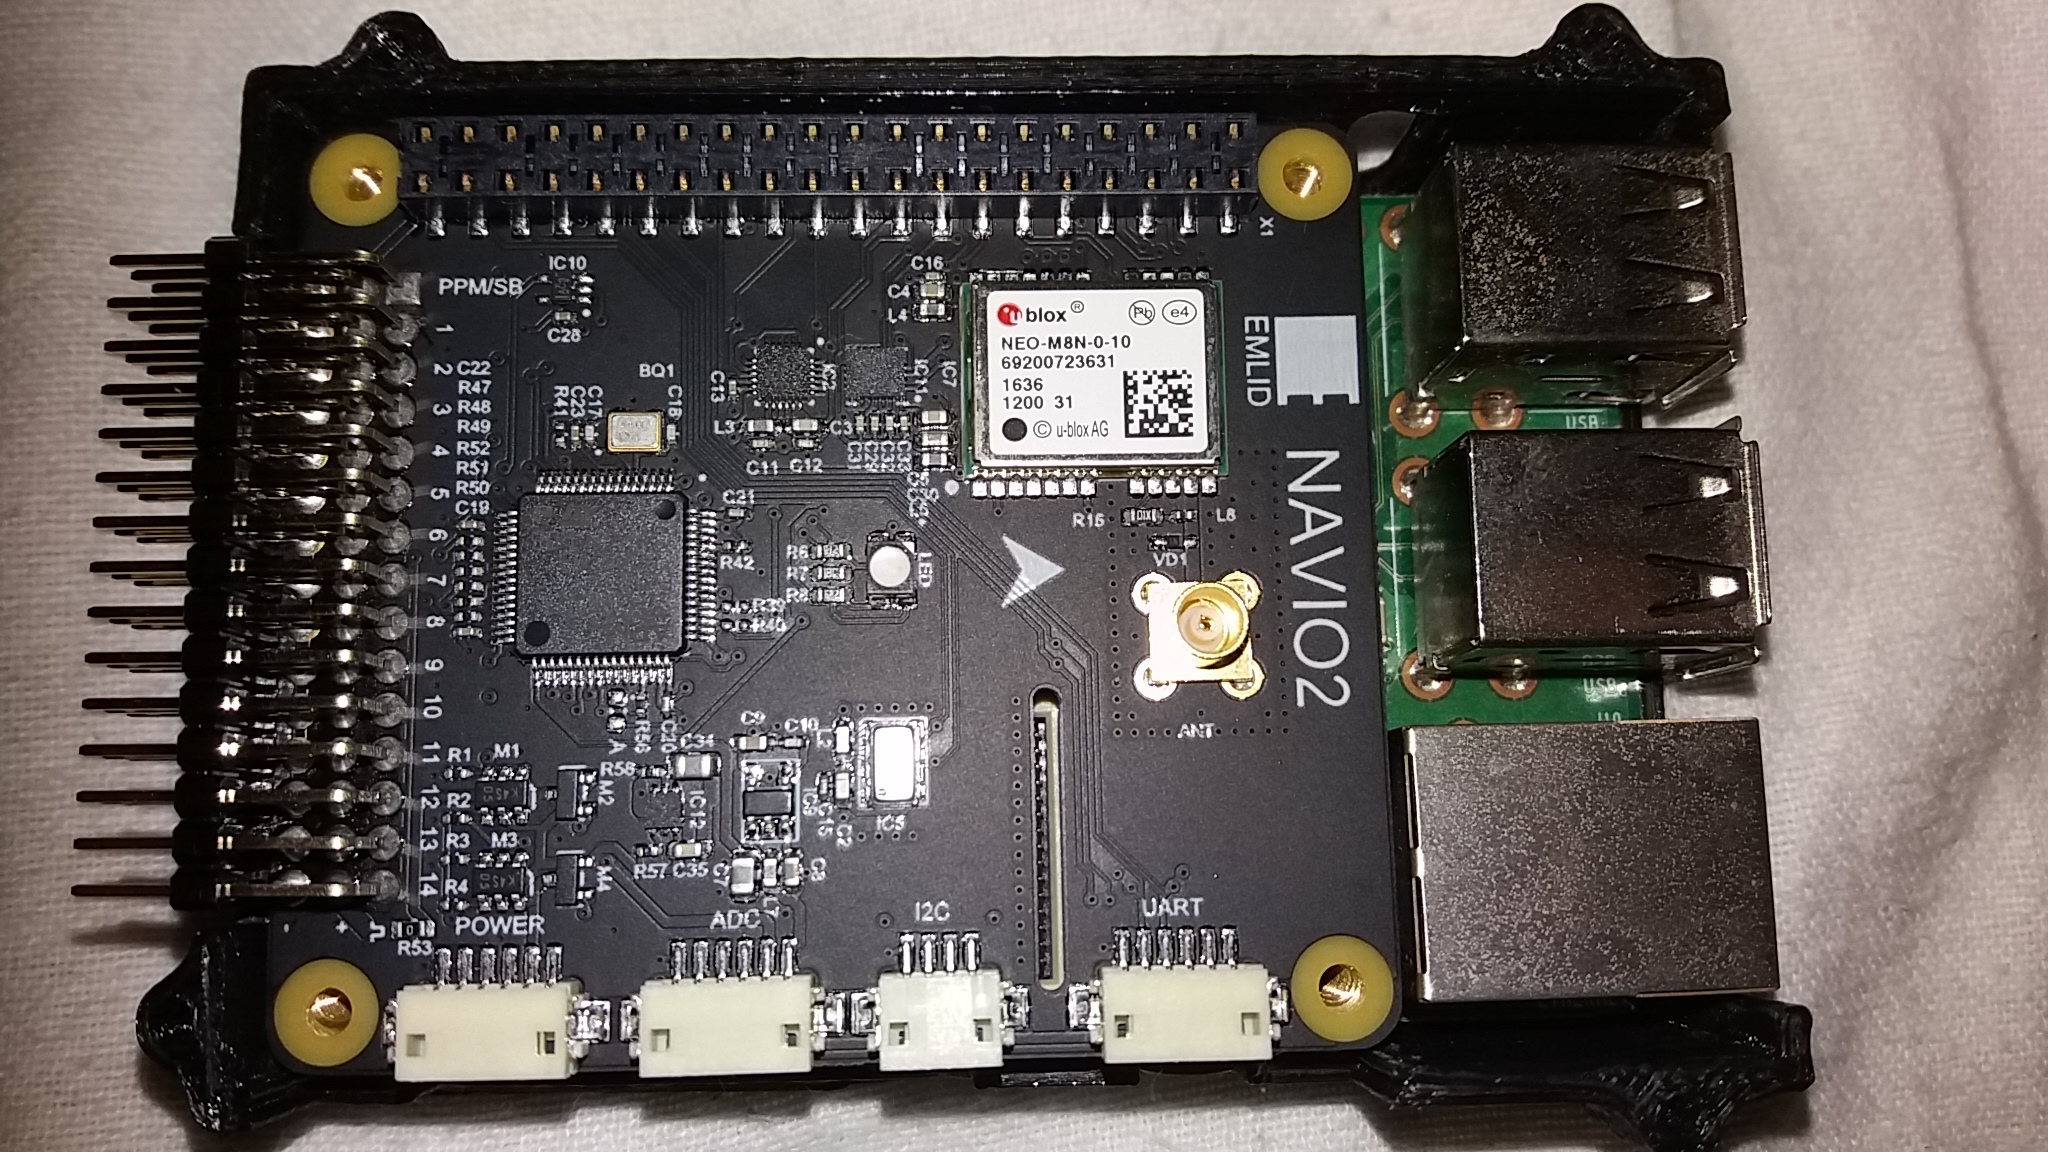
\includegraphics[scale=0.1]{images/drone-build-3dcase-pi-navio.jpg}
\caption{Fitting the Navio2 flight controller on top.}
\label{fig:insertion_navio}
\end{subfigure}
\caption{Inserting the sensitive electronics.}
\label{fig:insertion}
\end{figure}

\noindent
The Navio2 flight controller fits perfectly onto the Raspberry Pi's 40-pin header in Figure \ref{fig:insertion_navio}. It also uses every signal pin, except for one. The Navio2 communicates directly with the Broadcom CPU on the Pi, resulting in a multi-processor system. The greatest significance in this case is that flight variables can be monitored and controlled. It is non-trivial in standalone flight controllers, as the on-board firmware has to be modified with utmost care.

\begin{figure}[H]
\begin{subfigure}{0.5\textwidth}
\centering
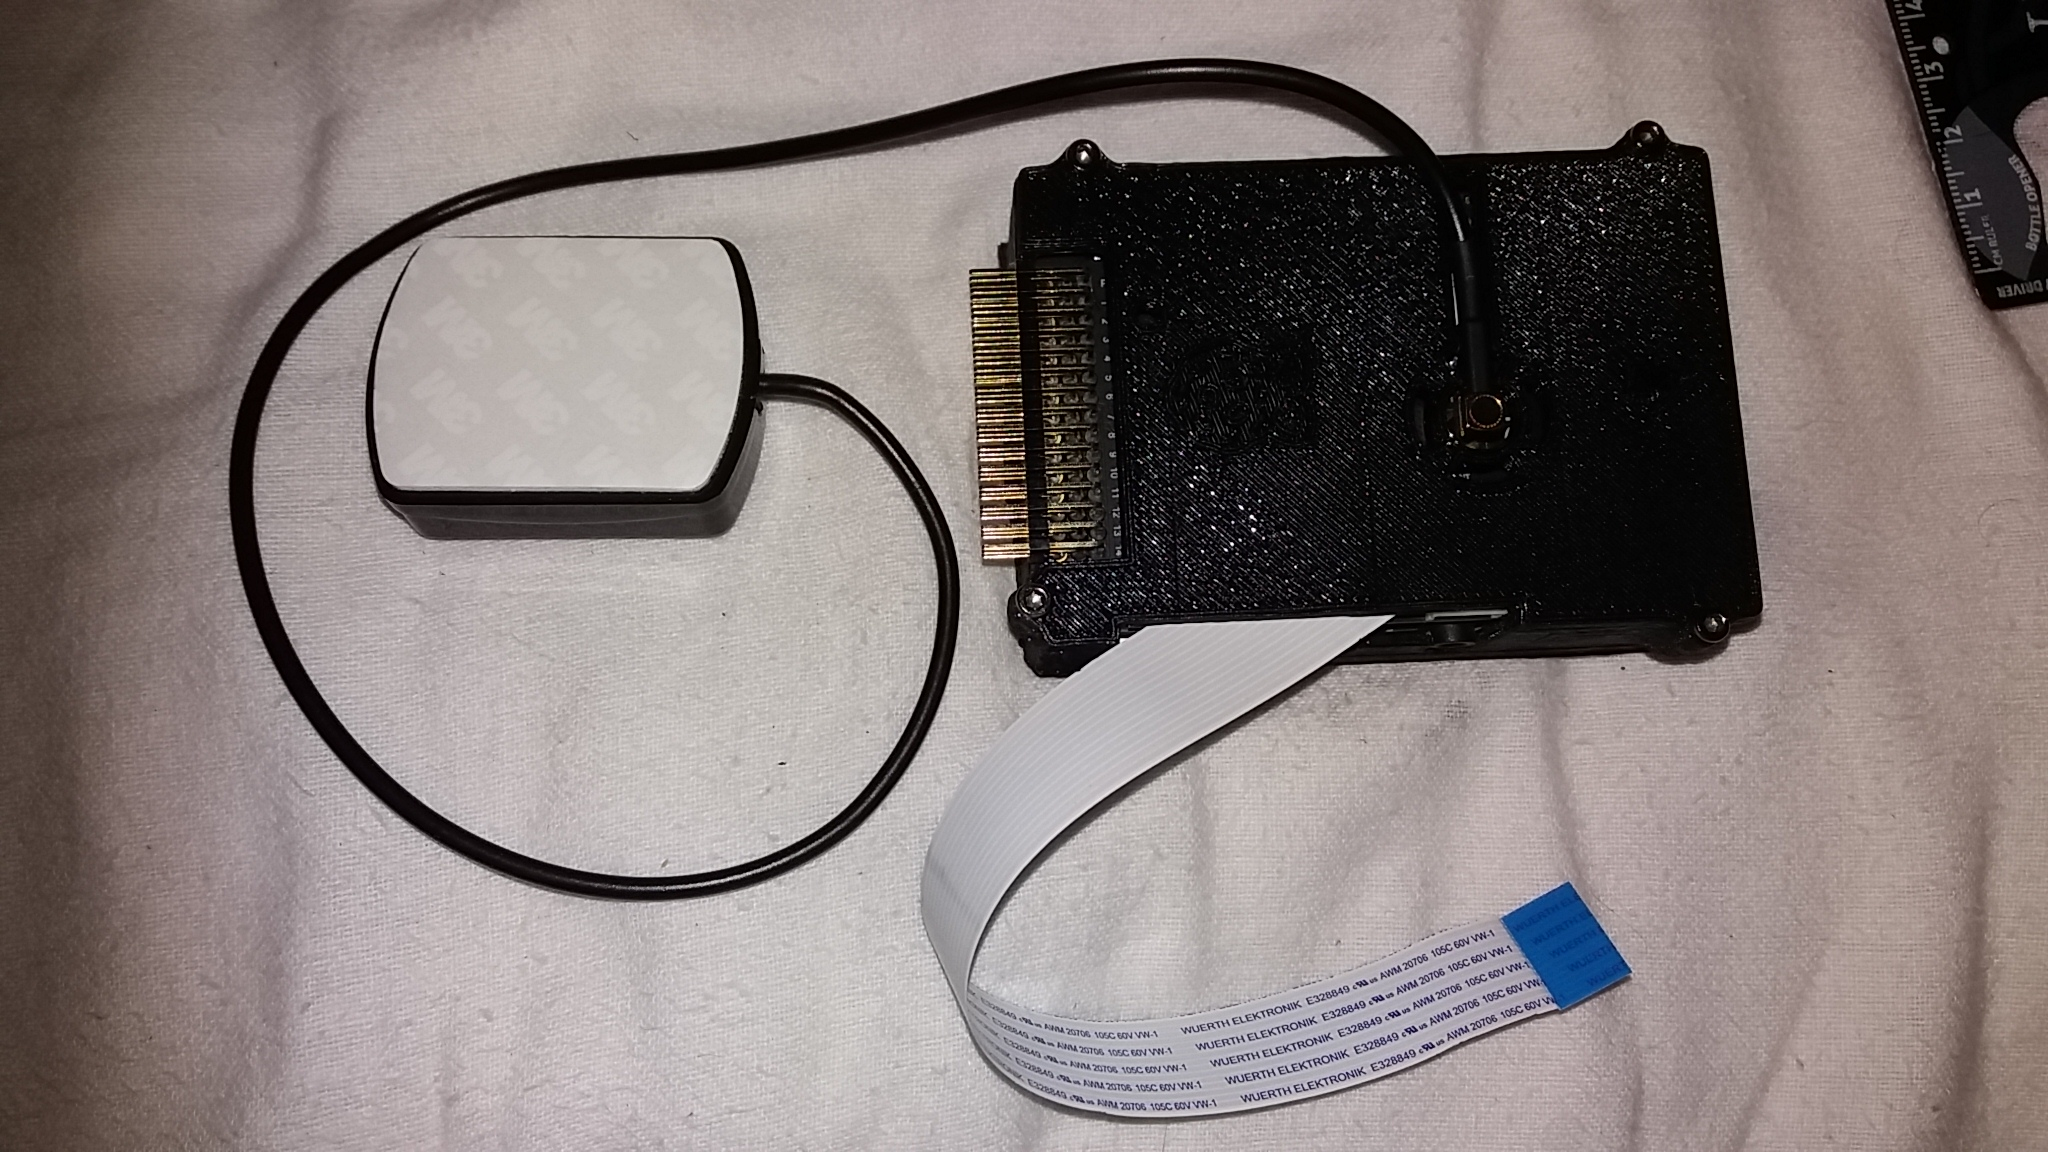
\includegraphics[scale=0.1]{images/drone-build-3dcase-gps.jpg}
\caption{Connecting Ublox Neo-7 GPS antenna and 15-pin camera CSI ribbon cable.}
\label{fig:stab_gps}
\end{subfigure}
\begin{subfigure}{0.5\textwidth}
\centering
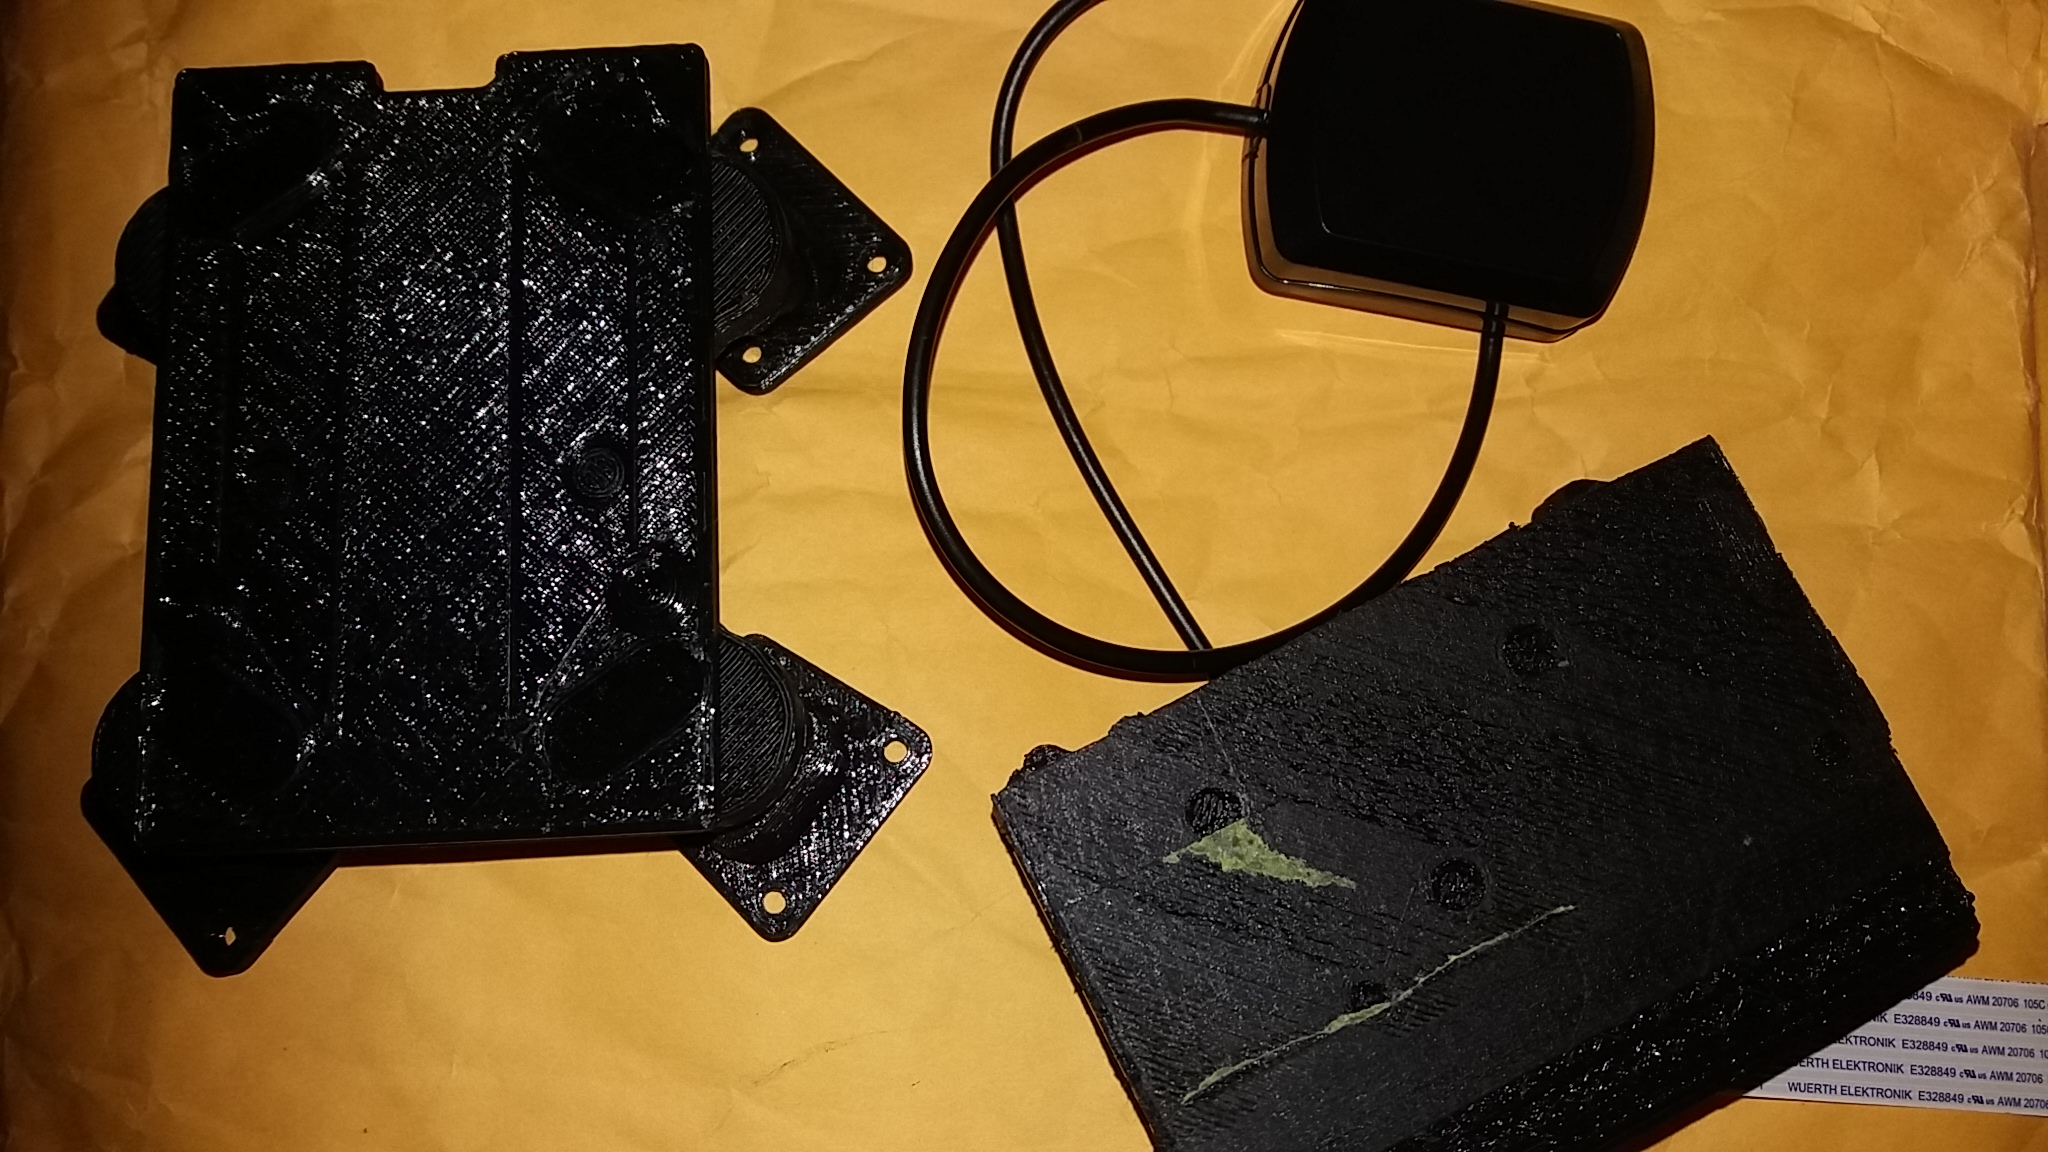
\includegraphics[scale=0.1]{images/drone-build-3dplatform.jpg}
\caption{Case and platform}
\label{fig:stab_case_plat}
\end{subfigure}
\caption{Putting the case and platform together}
\label{fig:stabilize_platform}
\end{figure}

\noindent
The GPS antenna lead fits snugly onto an SMA connector in Figure \ref{fig:stab_gps}, and is exposed in such a way as to leave enough freedom for the cable to bend, but not wear as if it were rigidly attached.

\begin{figure}[H]
\begin{subfigure}{0.5\textwidth}
\centering
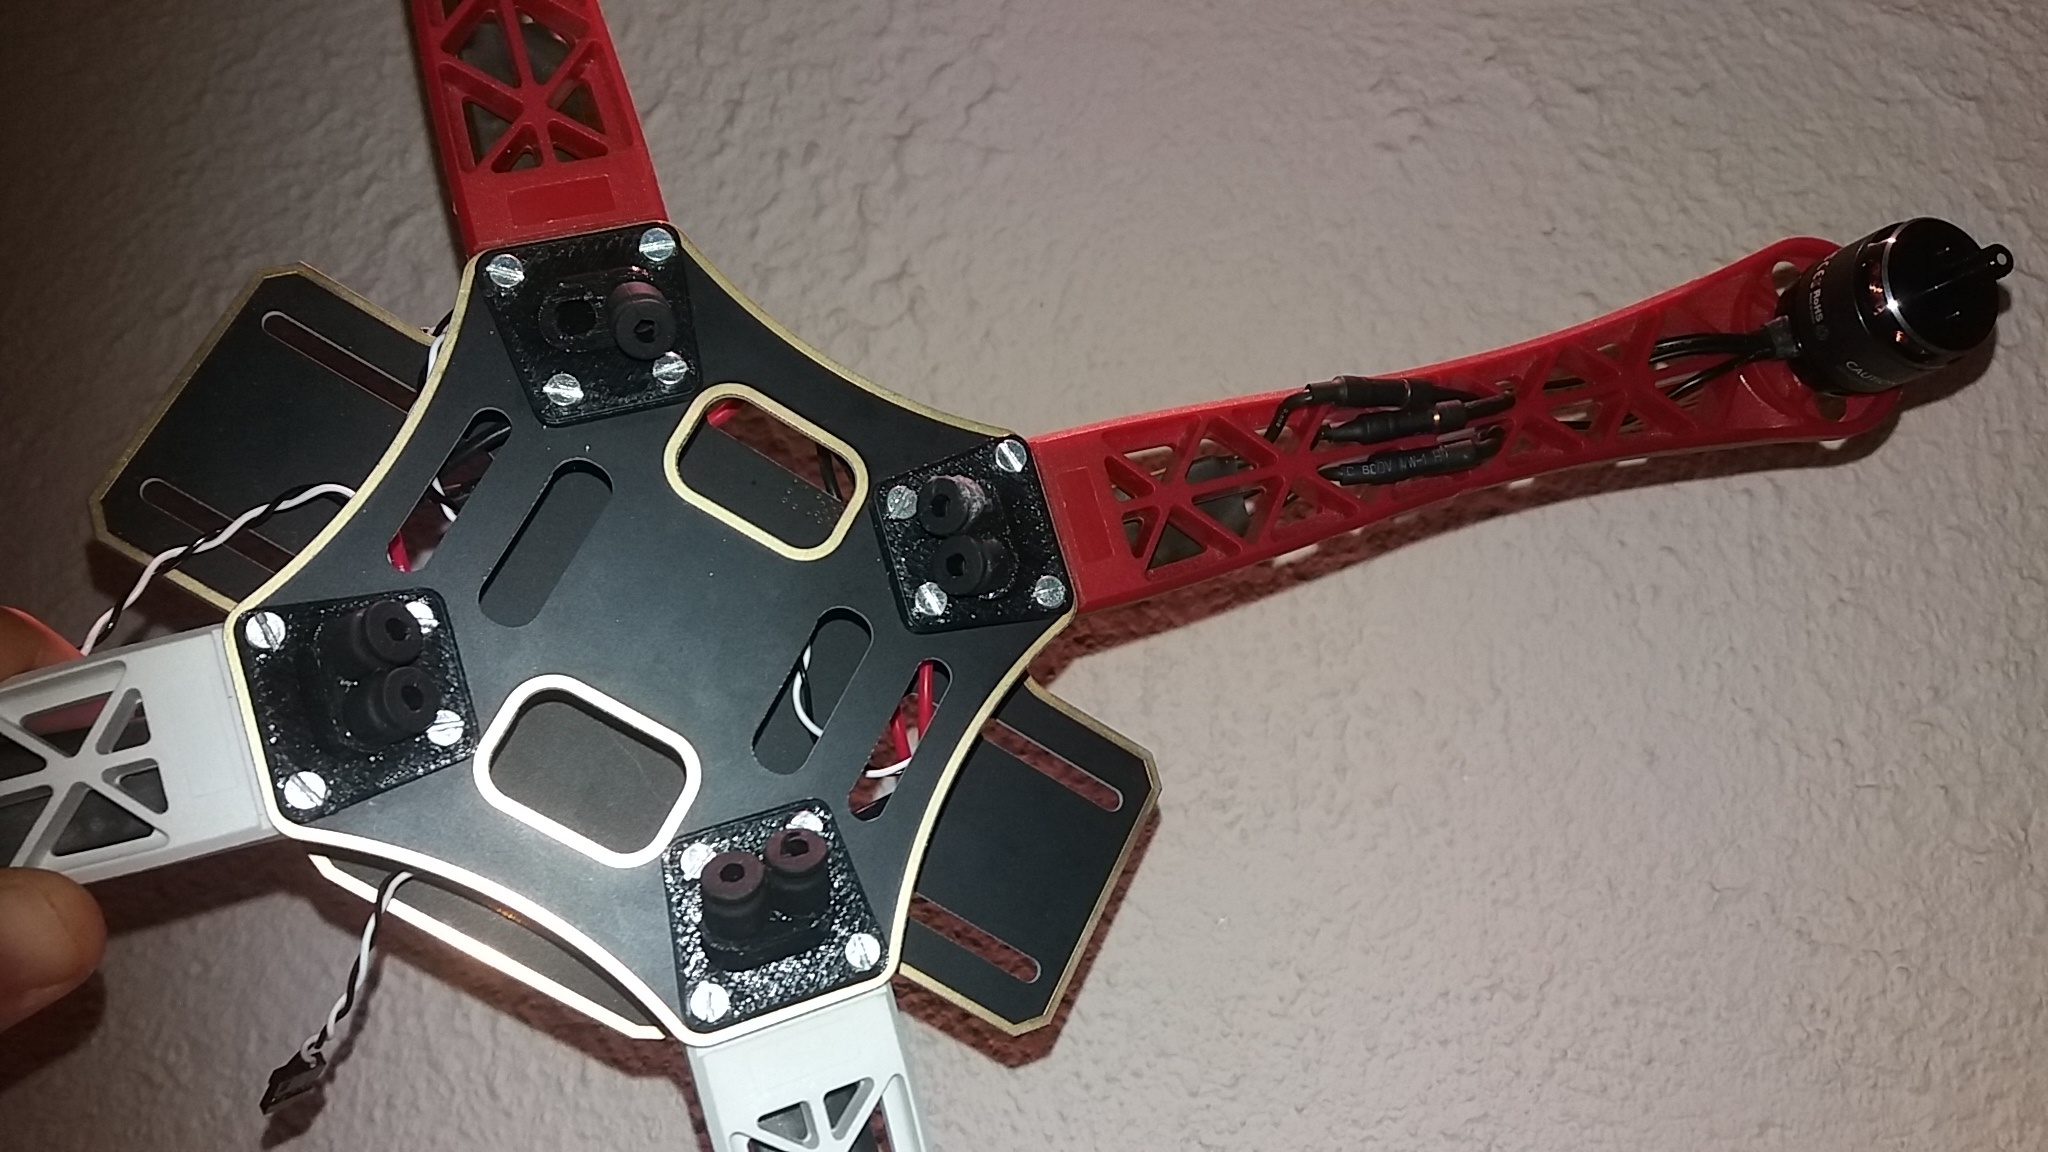
\includegraphics[scale=0.1]{images/drone-build-feet.jpg}
\caption{Added feet for platform.} 
\label{fig:feet}
\end{subfigure}
\begin{subfigure}{0.5\textwidth}
\centering
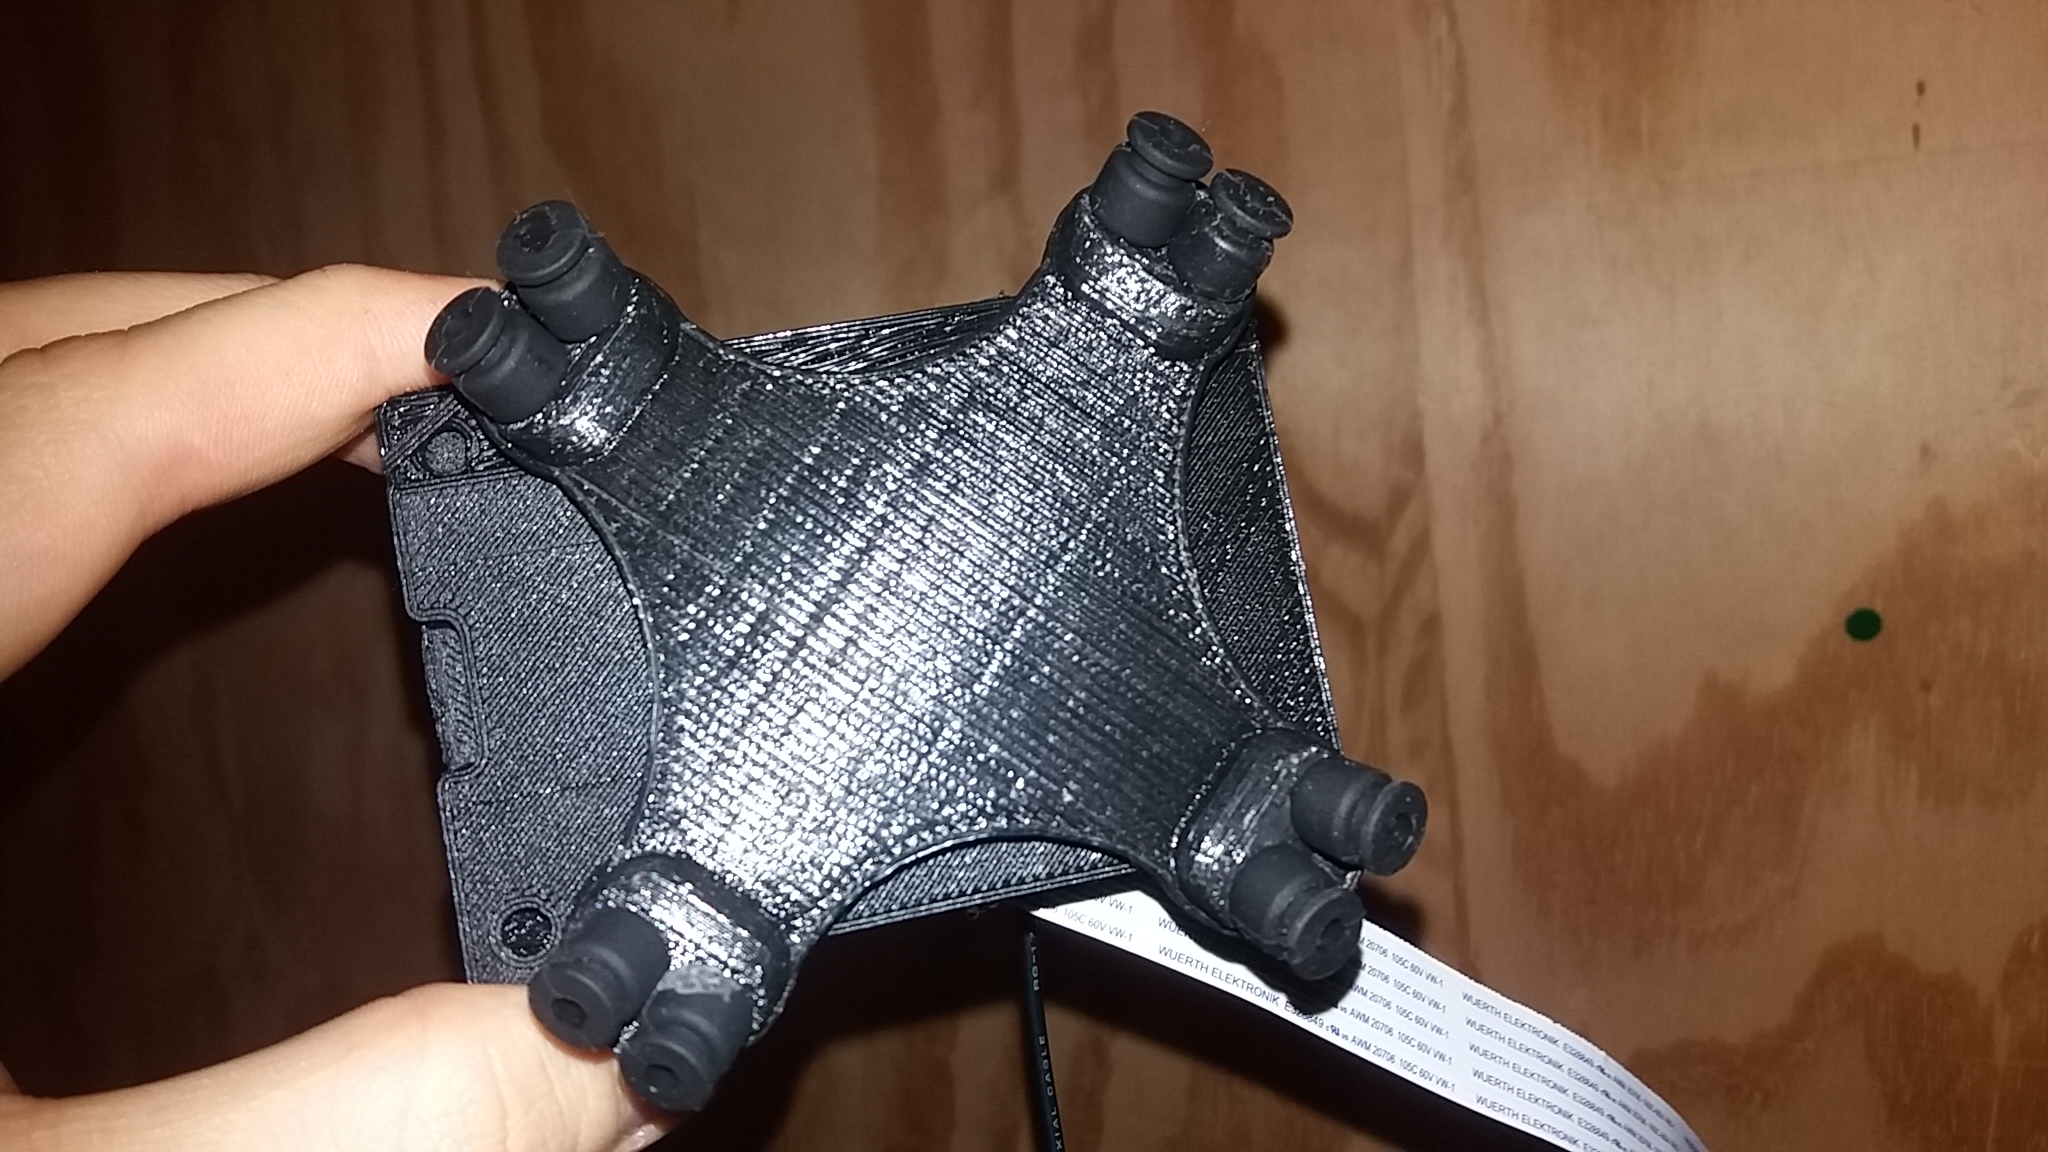
\includegraphics[scale=0.1]{images/drone-build-damper-balls.jpg}
\caption{Rubber vibration damper balls for platform.}
\label{fig:balls}
\end{subfigure}
\caption{Isolating vibrations between flight controller and the rest of the drone}
\label{fig:stabilize_platform}
\end{figure}

\noindent
One of the biggest problems in a drone is the vibrations emanating from the motors, travelling along the frame and affecting the flight controller. If not isolated from the flight controller, they induce a disturbance to the PID loop since the accuracy of the gyroscope, accelerometer and barometer readings are affected. In some cases, disturbed more than the PID loop can reasonably determine the current state of the drone.\\

\noindent
Thus, damper balls can be used to isolate vibrations significantly from the flight controller.

\begin{figure}[H]
\begin{subfigure}{0.5\textwidth}
\centering
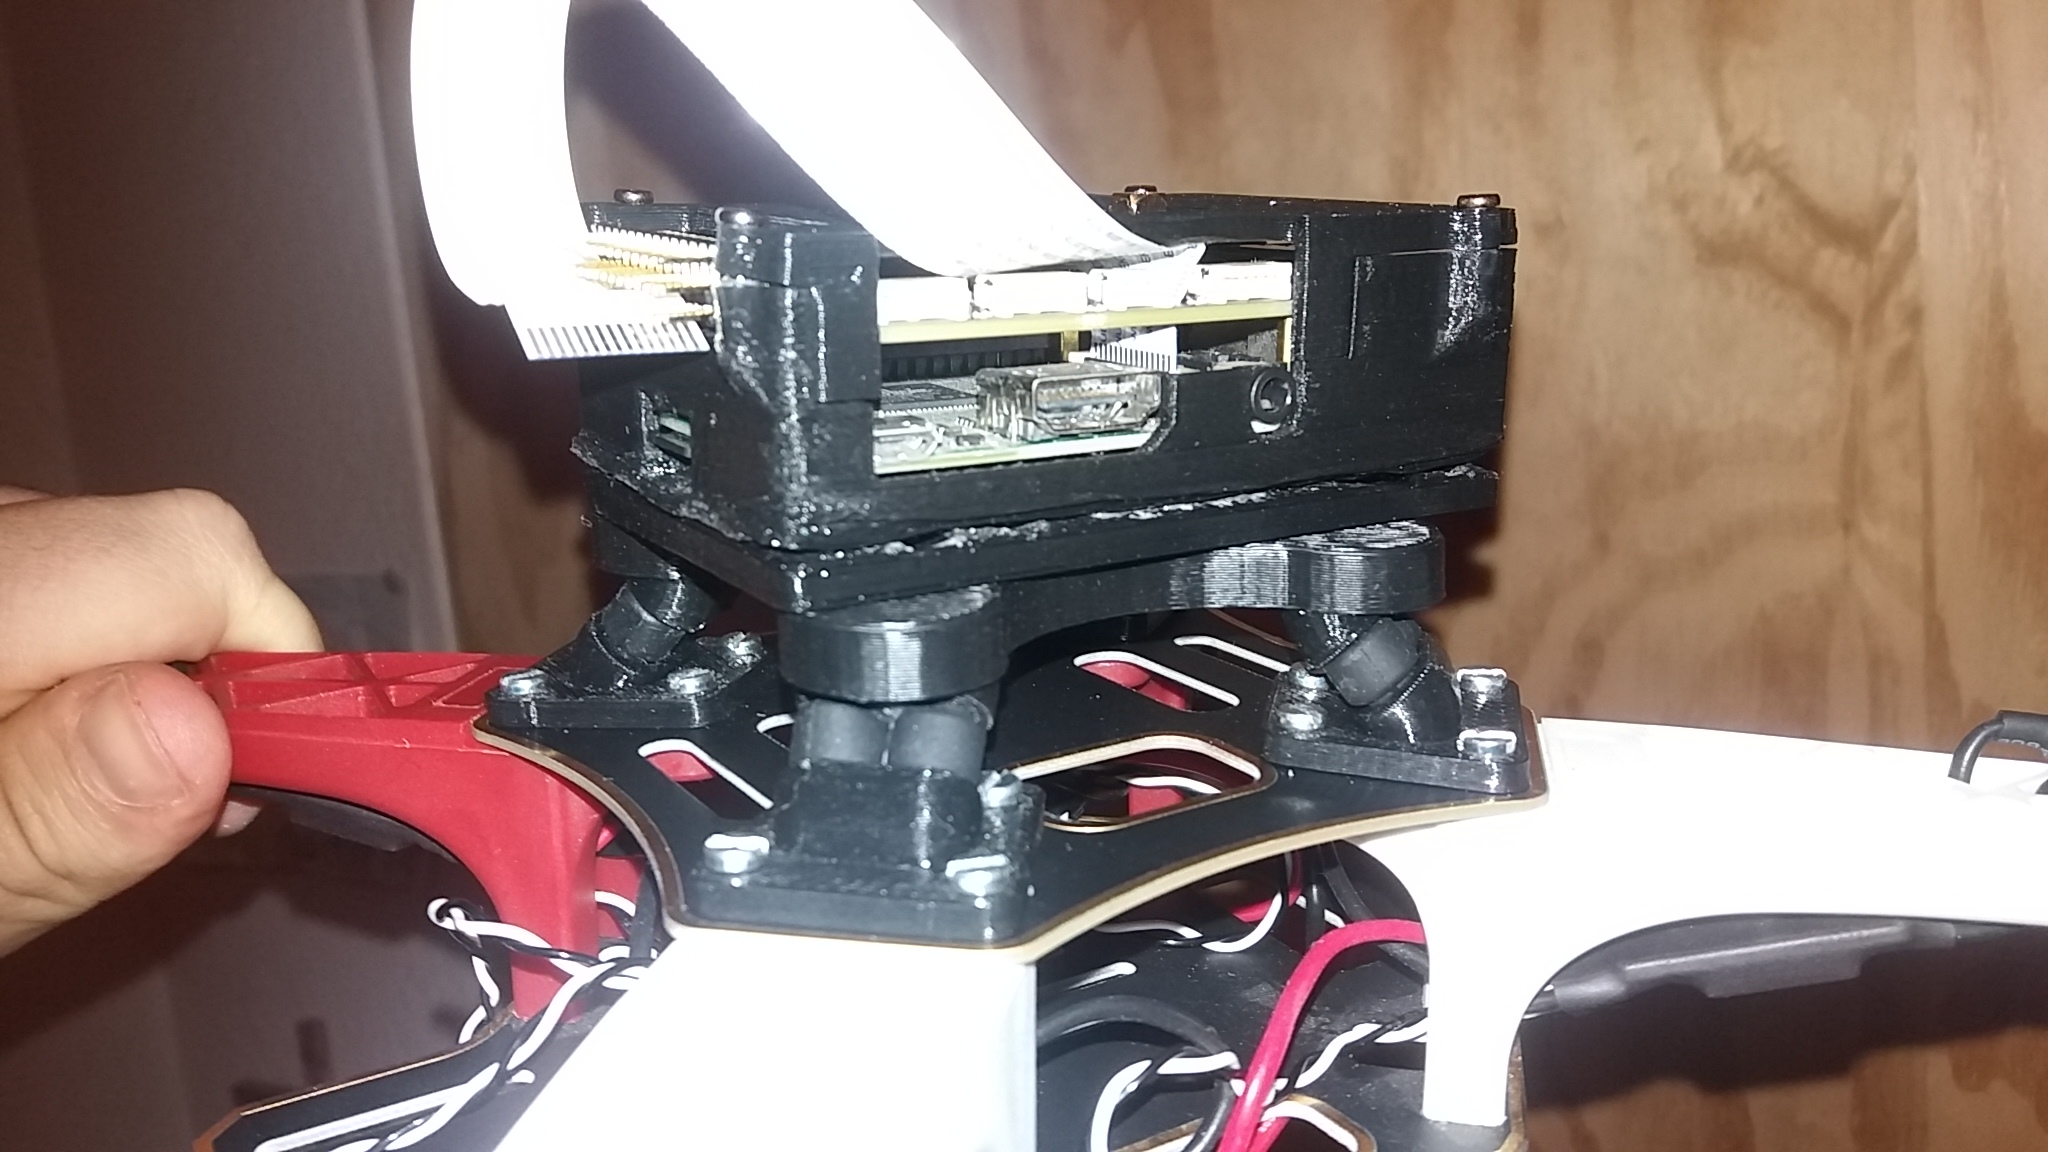
\includegraphics[scale=0.1]{images/drone-build-case-ondrone.jpg}
\caption{Attaching 3D printed case and platform to drone.}
\label{fig:attach_case_drone}
\end{subfigure}
\begin{subfigure}{0.5\textwidth}
\centering
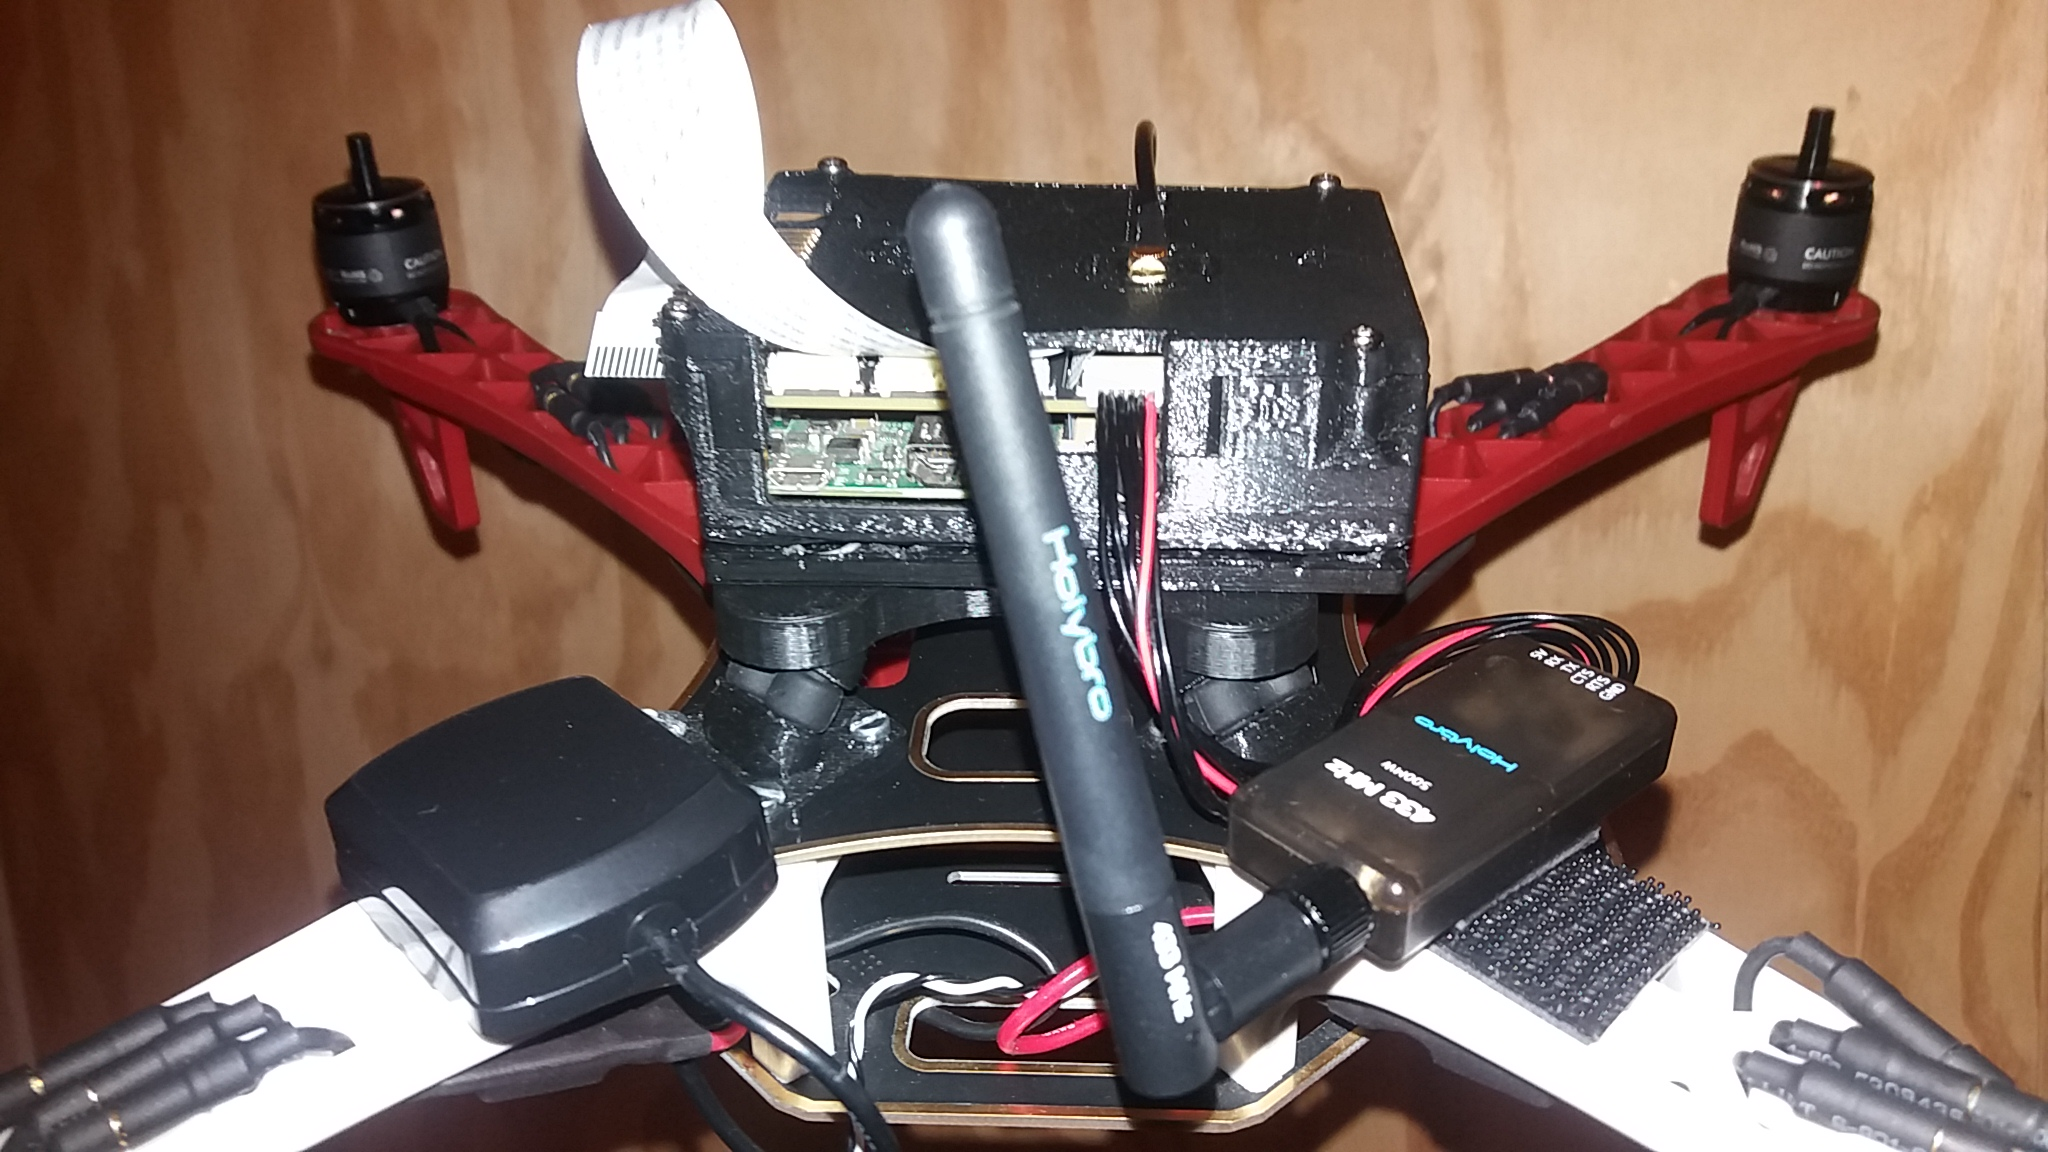
\includegraphics[scale=0.1]{images/drone-build-433.jpg}
\caption{Adding 433MHz telemtery to drone.}
\label{fig:attach_433}
\end{subfigure}
\caption{Isolating vibrations between flight controller and the rest of the drone}
\label{fig:attach_case_433}
\end{figure}

\noindent
Finally, the 3D printed enclosure is attached to the drone in Figure \ref{fig:attach_case_drone}. Also, the drone can communicate via wifi as its medium of wireless telemetry; but the interference from other devices in the crowded 2.4 GHz ISM band drastically reduces range -- especially from the handheld remote controller. That, and the dongles I had available seemed to work only for about 10 m.\\

\noindent
Thus, I connected a 433 MHz 100mW transceiver that communicates at 56400 baud to the GCS as in Figure \ref{fig:attach_433}. Real-time telemtery to a ground station is useful for pre-flight checks, in-flight monitoring and control, and missions.

\begin{figure}[H]
\begin{subfigure}{0.5\textwidth}
\centering
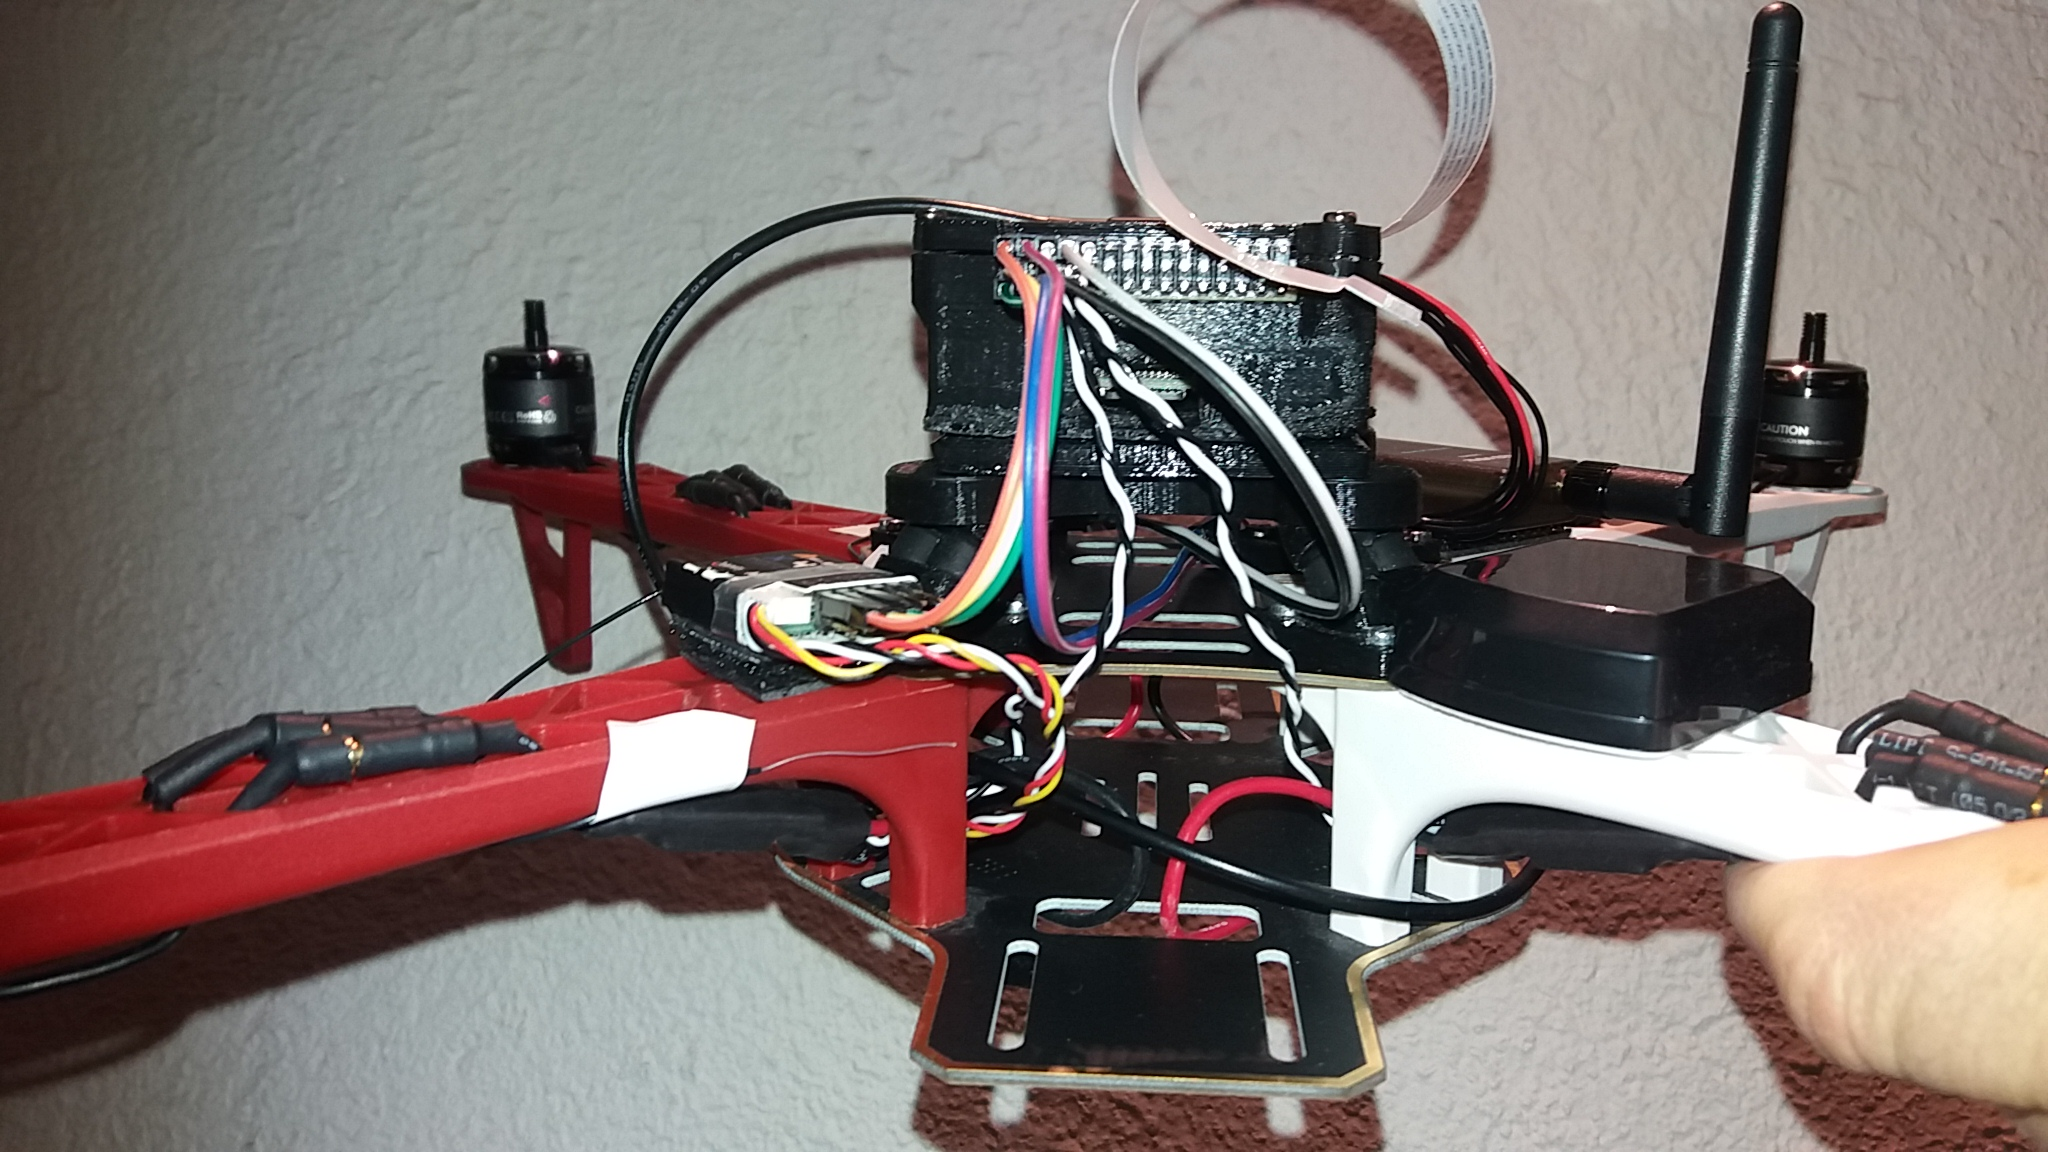
\includegraphics[scale=0.1]{images/drone-build-signal-wires.jpg}
\caption{Wiring up the signal wires}
\label{fig:attach_sbus}
\end{subfigure}
\begin{subfigure}{0.5\textwidth}
\centering
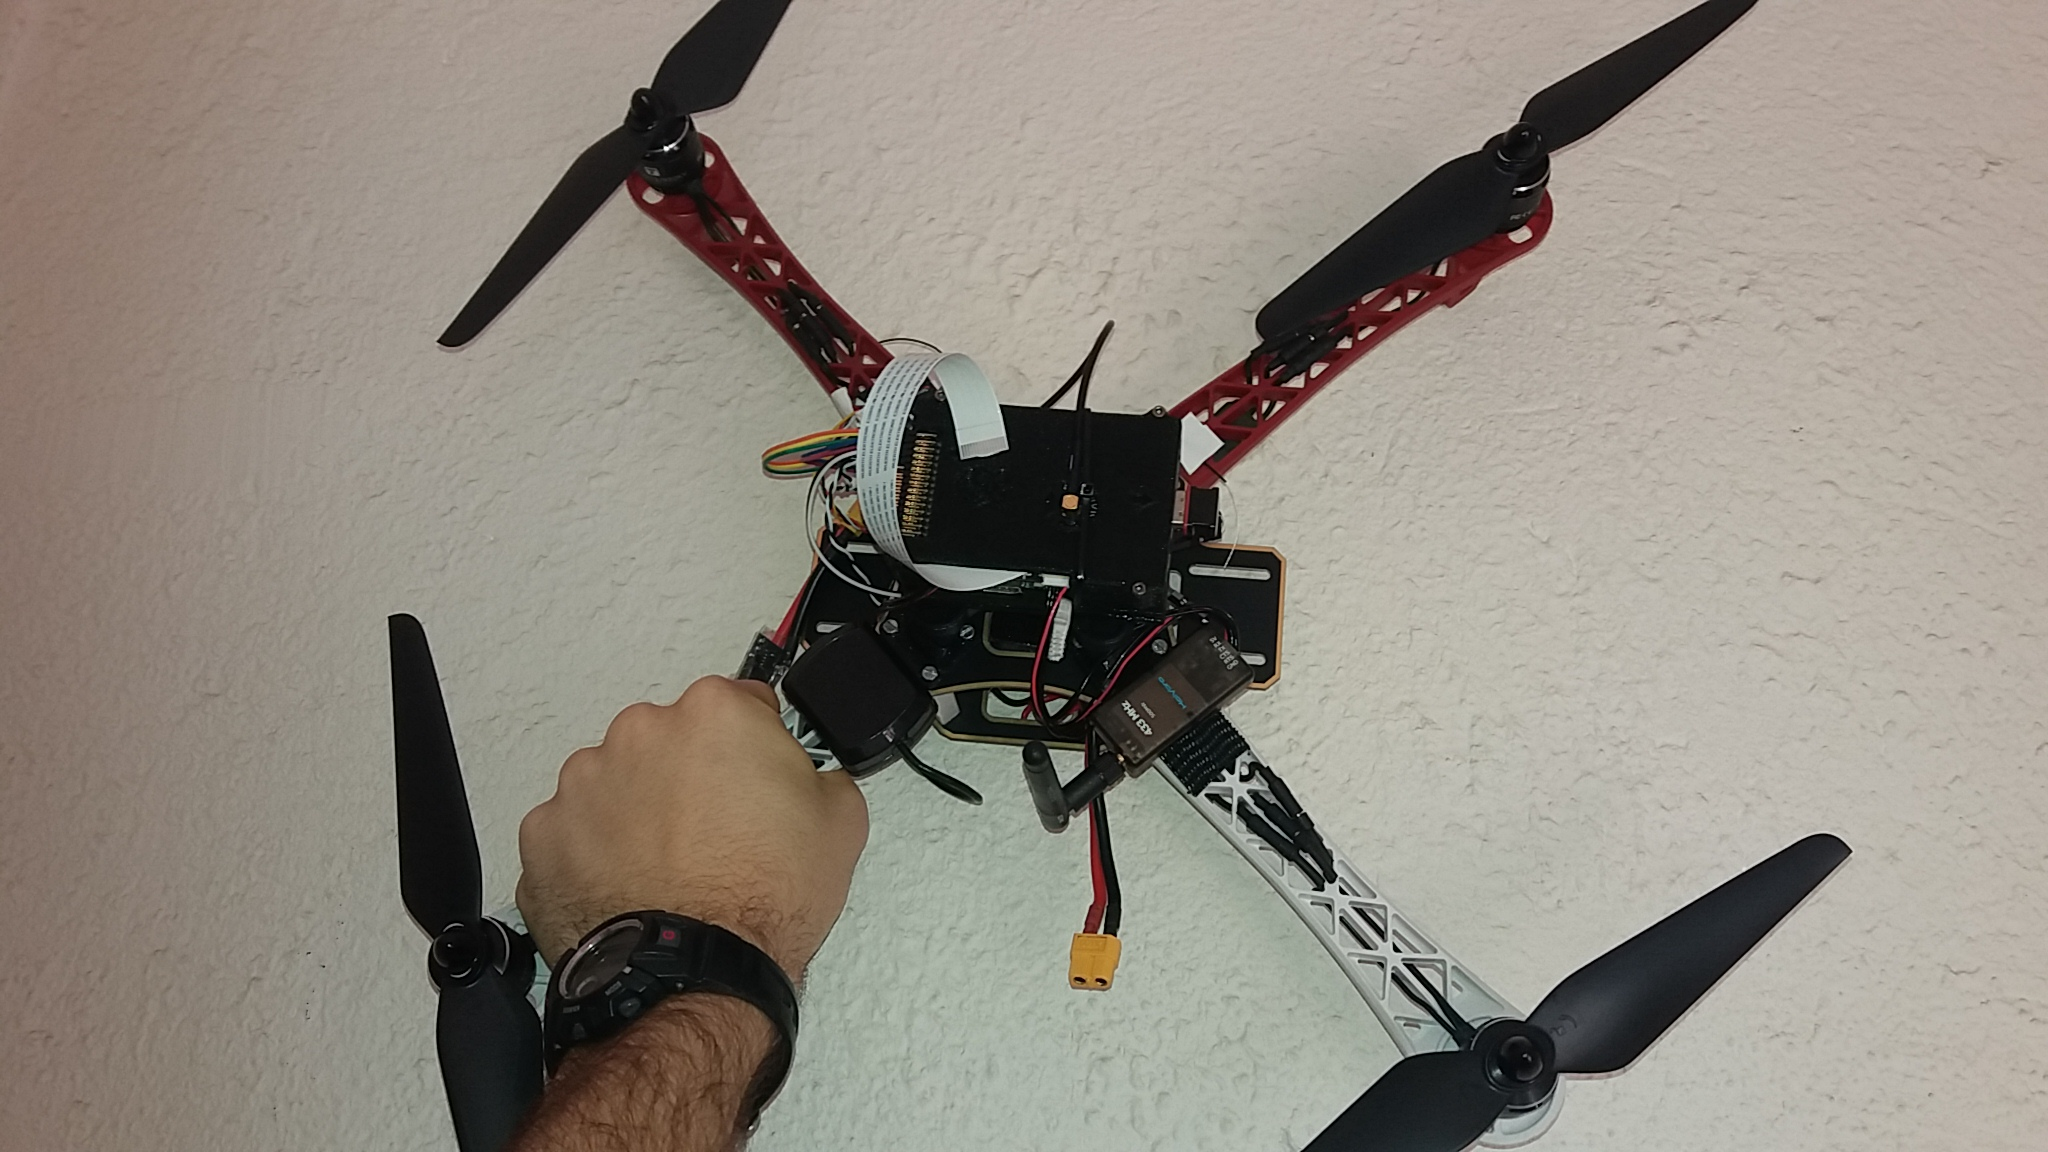
\includegraphics[scale=0.1]{images/drone-build-props.jpg}
\caption{Adding the 9.5'x4.5' propellers}
\label{fig:attach_props}
\end{subfigure}
\caption{Ready to fly}
\label{fig:attach_signal_props}
\end{figure}

The drone communicates with the handheld remote controller via S-BUS, which is a universal standard. The beauty of it is that it communicates with one signal wire as in Figure \ref{fig:attach_sbus}. Previous implementations one may have had to use pulse position modulation (PPM), where each channel requires a wire. Even though this may sound simple, it does increase PCB size, complexity and cost in the end.\\

\noindent
One the other hand, each electronic speed controller (ESC) gets a signal wire and power input.

\noindent
The propellers have a pitch of 4.5', which is basically a measure of the 'bite', or distance it travels through the air on one revolution.

\section{Ground Control Station}

Laptop, 433 MHz.

\section{Handheld transceiver}

Full-duplex transceiver returns battery and signal strength information, with the capability of sending other sensor data via serial.